\documentclass[a4paper,10pt]{ctexart}
%引用设置使用Bibtex
\usepackage{gbt7714}
\bibliographystyle{gbt7714-numerical}
%页面设置
\usepackage{geometry}
%字体设置
\usepackage{fontspec}
%\setmainfont{Times New Roman}
%定理环境
\usepackage{amsmath}
\numberwithin{equation}{section}
\usepackage{amsthm}
\newtheorem*{definition}{Definition}
\newtheorem{theorem}{Theorem}
\newtheorem{lemma}{Lemma}
\newtheorem*{corollary}{Corollary}
\newtheorem*{proposition}{Proposition}
\newtheorem*{example}{Example}
%数学环境字体
\usepackage{bm}
\usepackage[all]{xy}
%加载 TikZ 用于绘制交换图
\usepackage{tikz-cd}
\usepackage{tikz}
\usepackage{pgfplots}
\newcommand{\tikzdef}{\pgfmathsetmacro} % 在tikzpicture内的foreach循环中定义实数临时变量
%颜色
\usepackage{color,xcolor}

\definecolor{miku}{RGB}{57,197,187}
\definecolor{sakura}{RGB}{255,192,203}
\definecolor{rose}{RGB}{255,228,225}
\definecolor{brown}{RGB}{210,105,30}
\definecolor{lbrown}{RGB}{239,235,224}
\definecolor{bule}{RGB}{0,47,167}
\definecolor{lyellow}{RGB}{250,250,210}
\definecolor{lpurple}{RGB}{255,240,245}
\definecolor{lbule}{RGB}{135,206,250}
\definecolor{gbule}{RGB}{64,224,208}
\definecolor{green}{RGB}{138,200,207}
\definecolor{lgreen}{RGB}{225,255,255}
\definecolor{lorange}{RGB}{248,172,140}
\definecolor{salmon}{RGB}{250,128,114}
\definecolor{burgundy}{rgb}{0.5, 0.0, 0.13}
%链接设置
\usepackage[colorlinks=true,pdfstartview=FitH,linkcolor=blue,anchorcolor=violet, citecolor=magenta]{hyperref} 
%封面
\usepackage{pdfpages}
\usepackage{mathrsfs}
\usepackage{amssymb}
\usepackage{graphicx}
\usepackage{lipsum}
%彩色框
\usepackage{framed}
\usepackage{tcolorbox}
\tcbuselibrary{breakable}
\tcbuselibrary{theorems}
\tcbuselibrary{skins}
\usepackage{colortbl}
\usepackage{float}
\usepackage[export]{adjustbox}
\newtcolorbox[auto counter,number within=section]{notebox}[2][]{%
colback=miku!2!white,
colframe=miku,
coltitle=white,
fonttitle=\bfseries,
rightrule=2pt,
leftrule=2pt,
bottomrule=2pt,
colbacktitle=miku,
theorem style=standard,
breakable,
arc=2pt,
drop fuzzy shadow=black!20!white,
title=Note~\thetcbcounter: #2,#1}
\newtcolorbox[auto counter,number within=section]{markbox}[2][]{%
colback=miku!2!white,
colframe=miku,
coltitle=white,
fonttitle=\bfseries,
rightrule=0pt,
leftrule=0pt,
bottomrule=2pt,
colbacktitle=miku,
theorem style=standard,
breakable,
arc=0pt,
drop fuzzy shadow=black!20!white,
title=Remark~\thetcbcounter: #2,#1}
\newtcolorbox[no counter]{theorems}[2][]{%
width=12cm,
center,
sidebyside,
sidebyside adapt=left,
sidebyside gap=6mm,
sidebyside align=center seam,
colback=burgundy!2!white,
colframe=burgundy,
coltitle=white,
fonttitle=\bfseries,
rightrule=1pt,
leftrule=1pt,
bottomrule=2pt,
colbacktitle=burgundy,
theorem style=standard,
enhanced,
drop fuzzy shadow southeast=black!30!white,
breakable,
arc=0pt,
title=Theorem. #2,#1}
\newtcolorbox[no counter]{definitions}[2][]{%
width=12cm,
center,
colback=lyellow!2!white,
colframe=yellow!3!lyellow,
coltitle=bule,
fonttitle=\bfseries,
rightrule=0pt,
leftrule=1pt,
bottomrule=2pt,
colbacktitle=lyellow,
theorem style=standard,
breakable,
arc=5pt,
enhanced,
drop fuzzy shadow southeast=black!20!white,
title=Definition. #2,#1}
\newtcolorbox[auto counter,number within=section]{corollarys}[2][]{%
colback=lyellow!2!white,
colframe=lyellow,
coltitle=bule,
fonttitle=\bfseries,
rightrule=0pt,
leftrule=1pt,
bottomrule=2pt,
colbacktitle=lyellow,
theorem style=standard,
breakable,
arc=0pt,
enhanced,
drop fuzzy shadow southeast=black!20!white,
title=Corollary~\thetcbcounter: #2,#1}
\newtcolorbox[auto counter,number within=section]{lemmas}[2][]{%
width=12cm,
center,
colback=lyellow!2!white,
colframe=lorange!30!sakura,
coltitle=bule,
fonttitle=\bfseries,
rightrule=0pt,
leftrule=1pt,
bottomrule=2pt,
colbacktitle=lorange!30!sakura,
theorem style=standard,
breakable,
arc=5pt,
enhanced,
drop fuzzy shadow southeast=black!20!white,
title=Lemma. #2,#1}
\newtcolorbox[auto counter,number within=section]{propositions}[2][]{%
width=12cm,
center,
colback=salmon!5,
colframe=salmon!90!black,
coltitle=white,
fonttitle=\bfseries,
rightrule=1pt,
leftrule=1pt,
bottomrule=2pt,
colbacktitle=salmon!90!black,
theorem style=standard,
breakable,
arc=5pt,
enhanced,
drop fuzzy shadow southeast=black!20!white,
title=Proposition. #2,#1}
\newtcolorbox[no counter]{egbox}[2][]{%
width=12cm,
center,
colback=black!5!white,
colframe=black!20!white,
coltitle=black,
fonttitle=\bfseries,
rightrule=1pt,
leftrule=1pt,
bottomrule=2pt,
colbacktitle=black!20!white,
theorem style=standard,
breakable,
arc=0pt,
enhanced,
drop fuzzy shadow southeast=black!20!white,
title=Example. #2,#1}

%\begin{figure}[H]
%\centering
%\includegraphics[center]{pic.png}
%\end{figure}
\geometry{left=3cm,right=3cm,top=2cm,bottom=2cm}
\tcbuselibrary{most}

\usepackage[linesnumbered,ruled,vlined]{algorithm2e}
\usepackage{algorithmic}

\SetKwProg{Fn}{function}{\string:}{}
\newcommand{\forcond}{$i=0$ \KwTo $n$}
\SetKwFunction{FRecurs}{FnRecursive}
\SetKwInput{KwCost}{Cost}

\usepackage{holtpolt}

%自定义设置
\renewcommand{\proofname}{Proof.}
\renewcommand{\contentsname}{ Content }
\newcommand{\image}[2]{
    \centering
    \includegraphics[width={#1}\textwidth]{#2}
}



\newcommand\keywords[1]{\vskip2ex\par\noindent\normalfont{\textbf{关键词}: #1}}
\newcommand{\ekeywords}[1]{\vskip2ex\par\noindent\normalfont{\bfseries Key Words: }#1}
\newcommand{\miku}{\textcolor{miku}}
\newcommand{\sakura}{\textcolor{sakura}}
\newcommand{\brown}{\textcolor{brow}}
\newcommand{\red}{\textcolor{red}}
\newcommand{\blue}{\textcolor{blue}}
\newcommand{\A}{\mathcal{A}}
\newcommand{\C}{\mathbb{C}}
\newcommand{\al}{\alpha}
\newcommand{\sa}{$\sigma$-algebra}
\newcommand{\Bsa}{Borel $\sigma$-algebra}
\newcommand{\F}{\mathcal{F}}
\newcommand{\N}{\mathcal{N}}
\newcommand{\M}{\mathcal{M}}
\newcommand{\m}{ $\mathcal{M}$ }
\newcommand{\B}{\mathcal{B}}
\newcommand{\myP}{\mathcal{P}}
\renewcommand{\bf}[1]{\textbf{#1}}

\newcommand{\myRom}[1]{\uppercase\expandafter{\romannumeral#1}}
\newcommand{\pl}{$ L^p(X) $}
\newcommand{\twol}{$ L^2(X) $}

\usepackage{booktabs}

\begin{document}
\hfill\vbox{\hbox{Numerical Analysis}\hbox{陈曦,UESTC}\hbox{Summer, 2024}}

\begin{center}\Large
    \textbf{数值线性代数}\\{\normalsize\bf {数值误差分析基础和线性系统的微扰}}
\end{center}
\vskip 30pt
\begin{center}
    \small {参考书目:Accuracy and Stability of Numerical Algorithms(Higham,2002)}
\end{center}

粗略地讲,数值分析包括两大部分:设计算法以及误差分析。针对某一具体问题,首先需要根据该问题的特点设计一个算法,然后对该算法的误差进行分析,以保证算法的正确性和稳定性。此外,当需要解决一个实际问题时,还需要考虑计算效率等问题。本文主要讨论误差分析这一部分。

\section{数值误差分析}
在数值计算中需要研究各种误差对于计算结果的影响,这些误差主要有三个来源:
\begin{itemize}
    \item 舍入(Rounding)——浮点计算;
    \item 截断(Truncation)——离散化;
    \item 数据自身(Data uncertainty)——测量误差。
\end{itemize}
其中舍入引起的误差可以通过浮点数系的分析来研究,截断则可以通过数值微分和数值积分的分析来研究并给出误差估计,最后,数据自身的误差对计算结果的影响取决于系统的敏感性和病态程度,这一部分的分析主要依赖于微扰论。通过引入前向和后向误差分析,我们可以将前两个误差造成的影响等价于对原系统的扰动,于是可以使用微扰论的方法来统一地分析这些误差对计算结果的影响。

\subsection{浮点数系}
数值计算的基础是浮点运算,这一节简要回顾浮点数系的基础知识。

一般地,一个浮点数形如
\begin{equation}
    y = \pm m\times \beta^{e-t},
\end{equation}
其中$ m $是\emph{主要部分}(Significand),要求$ 0\leqslant m\leqslant \beta^t-1 $,$ \beta $是\emph{基数}(Base),$ t $称为该浮点数系的\emph{精度}(Precision),指数$ e $满足$ e_{\min}\leqslant e\leqslant e_{\max} $(Exponent range)。除了以上形式,也可以使用其他的方式描述浮点数:
\begin{equation}
    y = \pm \beta^e\times \left( \frac{d_1}{\beta} + \frac{d_2}{\beta^2} + \cdots + \frac{d_t}{\beta^t} \right) = \pm \beta^e\times (0.d_1d_2\cdots d_t)_\beta.
\end{equation}
在这种表示方法中,$ m = (d_1d_2\cdots d_t)_\beta $。

由于指数的取值范围是有限的,浮点数可以被划分为两大类:\emph{正则浮点数}(normal number)和\emph{次正则浮点数}(subnormal number)。当$ e = e_{\min} $并且$ m = (0d_2\cdots d_t)_\beta $,即$ d_1=0 $时,称浮点数$ y=\pm \beta^{e_{\min}}\times (0.0d_2\cdots d_t)_\beta $是次正则的,其余的浮点数称为正则的。这样一个浮点数系内非零浮点数的取值范围为
\begin{equation}
    \beta^{e_{\min}-t}\leqslant |y|\leqslant \beta^{e_{\max}}(1-\beta^{-t}).
\end{equation}
如果试图使用这一浮点数系来表示这一范围之外的数,则会发生溢出,这包含\emph{上溢}(Overflow)和\emph{下溢}(Underflow)两种情况。在这一范围中,正则浮点数和次正则浮点数分别落在
\[
    \begin{aligned}
        \text{Normal: } & \beta^{e_{\min}-1}\leqslant |y|<\beta^{e_{\max}}(1-\beta^{-t}),\\
        \text{Subnormal: } & \beta^{e_{\min}-t}<|y|<\beta^{e_{\min}-1}.
    \end{aligned}
\]

接下来,为了描述某一浮点数系的精度,我们考虑最小的大于$ 1= \beta\times (0.10\cdots00)_\beta $的浮点数$ \beta\times (0.10\cdots01)_\beta $与$ 1 $之间的距离,即
\begin{equation}
    \varepsilon = \beta\times (0.00\cdots01)_\beta = \beta^{1-t}.
\end{equation}
称这一数值为该浮点数系的\emph{机器精度}(Machine epsilon)。以下我们使用$ fl(x) $表示经由某种舍入规则得到的$ x $的浮点值。可以证明如果$ x $落在浮点数系的表示范围内,即不发生溢出,则浮点表示的相对误差满足
\begin{equation}
    \frac{|fl(x)-x|}{|x|}\leqslant \frac{1}{2}\beta^{1-t} :=u
\end{equation}
上式右侧的值称为该数系的\emph{单位舍入误差}(Unit roundoff)。于是我们有
\begin{equation}
    fl(x) = (1+\delta_1)x = \frac{x}{1+\delta_2},\quad |\delta_{i}|\leqslant u, i=1,2.
\end{equation}
这一结果贯穿了整个数值计算的误差分析,是之后所有误差分析的基础。
另外,对任意浮点数$ y=\pm \beta^e\times (0.d_1d_2\cdots d_t)_\beta $而言,定义它的\emph{最后一位上的单位值}(Unit in the last place, ULP)为$ ulp(y) = \beta^{e-t} $,这是$ y $与距它最近的浮点数之间的距离。$ ulp $与机器精度$ \varepsilon $之间的关系为
\begin{equation}
    ulp(y) = \beta^{e-1}\cdot\varepsilon.
\end{equation}

使用浮点数表示代替某一准确值的过程称作舍入,在这一过程中引入的误差就称作舍入误差,该误差除了与浮点数系自身的精度有关外,还取决于使用的舍入规则。常用的舍入规则包括向零舍入,向无穷舍入,向上舍入,向下舍入,以及向最近舍入等。当采用\emph{向最近舍入}(Round to nearest)时,还必须考虑当准确值落在两个相邻的浮点数中央的情况,这时最常用的规则是\emph{偶数舍入}(Round to even),选取主要部分最后一个bit为0的浮点数为最终浮点表示。

为了在计算机上进行数值运算,除了要使用浮点数近似表示真实数据之外,我们还必须考虑浮点运算。为了使浮点运算具有与浮点表示一致的形式,即
\begin{equation}
    fl(x\odot y) = (x\odot y)(1+\delta_1) = \frac{x\odot y}{1+\delta_2},\quad |\delta_i|\leqslant u, i=1,2,
\end{equation}
(其中的$ \odot $可以是加减乘除) 在真实的计算机上,浮点数在储存时除了根据舍入规则进行舍入之外,还额外储存了一些特殊的bit来使上面的关系成立,例如为确保浮点加法和减法可以满足如上关系,通常需要借助3个额外的bit,其中两个bit被称作guard bit,另一个bit称作sticky bit,这些特殊bit用来使舍入可以正常进行。

目前最通用的浮点数系由IEEE 754标准规定,该数系使用2作为基数,其中单精度浮点数使用32bit表示,其中一个bit表示符号,23个bit用于表示主要部分$ m $,8个bit用于表示指数$ e $,$ t=24,e_{\min}=-125,e_{\max}=128 $;双精度浮点数使用64bit表示,类似地用一个bit表示符号,52个bit用于表示主要部分$ m $,11个bit用于表示指数$ e $,$ t=53,e_{\min}=-1021,e_{\max}=1024 $。两者都使用向最近舍入和偶数舍入。

\begin{figure}[htpb]
    \centering
    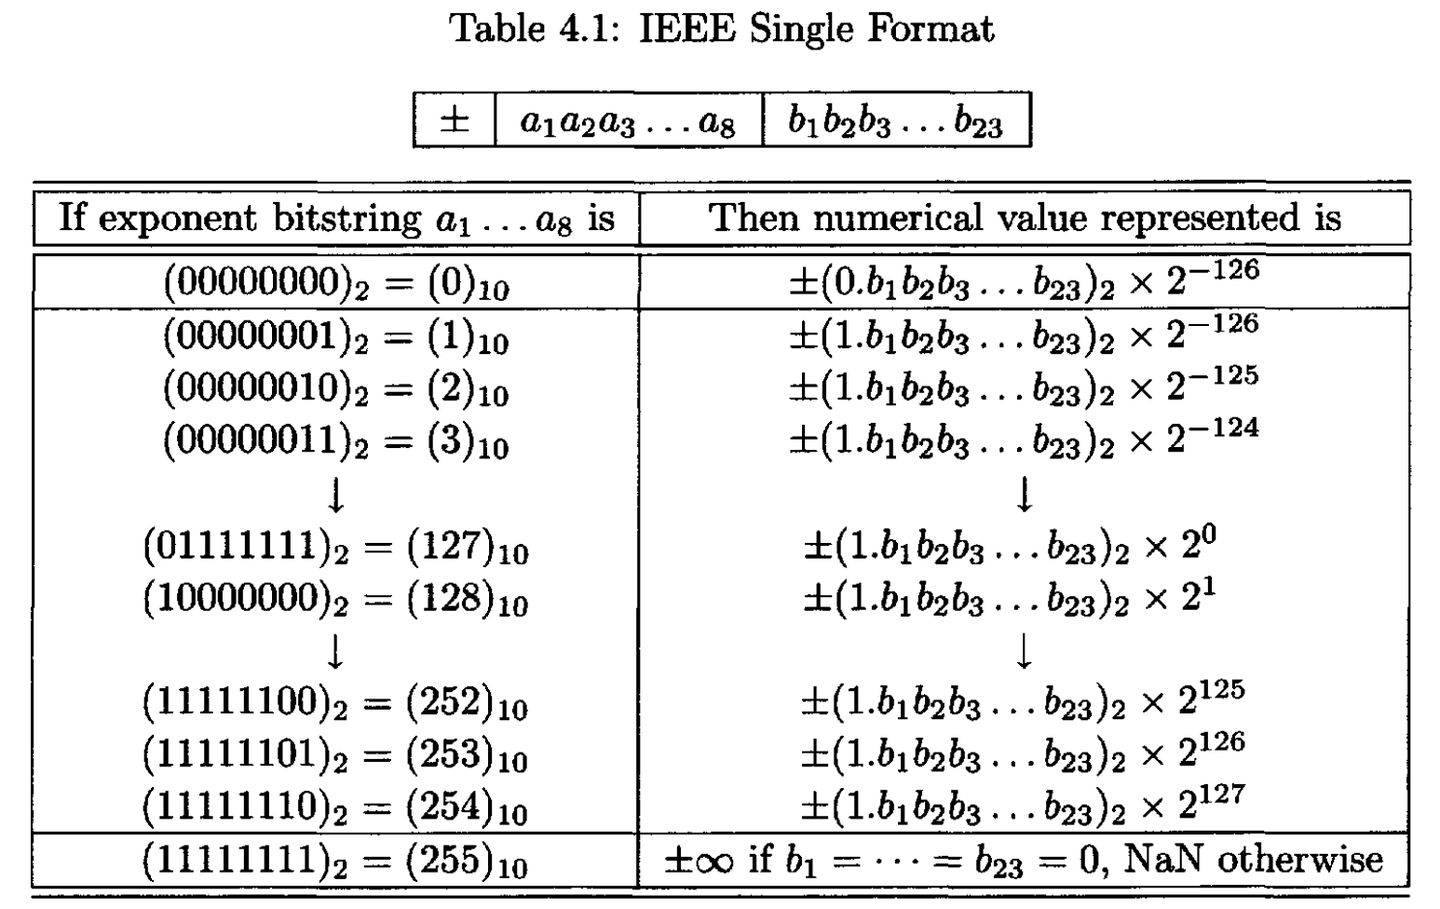
\includegraphics[width=0.8\textwidth]{IEEE Single Format.png}
    \caption{单精度浮点表示,来自Numerical Computing with IEEE Floating Point Arithmetic}
    \label{fig:SingleFormat}
\end{figure}

\begin{figure}[htpb]
    \centering
    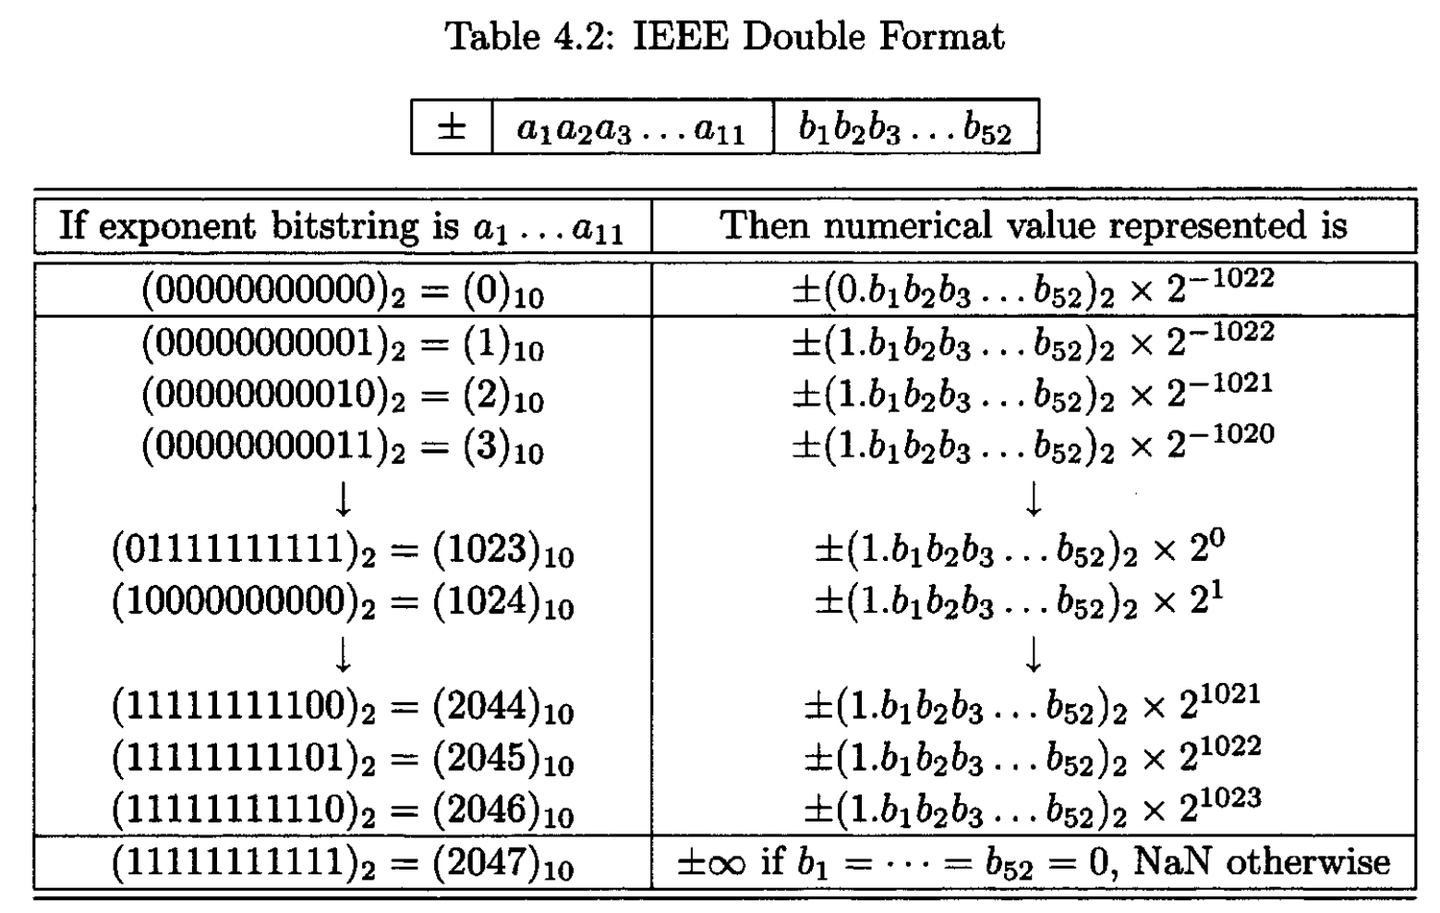
\includegraphics[width=0.8\textwidth]{IEEE Double Format.png}
    \caption{双精度浮点表示,来自Numerical Computing with IEEE Floating Point Arithmetic}
    \label{fig:DoubleFormat}
\end{figure}

两种数值格式的浮点表示如图\ref{fig:SingleFormat}和图\ref{fig:DoubleFormat}所示。从图中不难发现,采用2作为基数的好处之一是,如果使用本节开头的表示$ y = \pm \beta^e \times (0.d_1d_2\cdots d_t) $,则当$ e = e_{\min} $时,$ d_1=0 $,而当$ e > e_{\min} $时,$ d_1=1 $,即$ d_1 $被指数$ e $完全确定,所以无需储存$ d_1 $,这一节省下来的bit可以被用于储存符号($ d_1 $对应于图\ref{fig:SingleFormat}和图\ref{fig:DoubleFormat}中右栏小数点前面的0或者1)。如果使用单精度格式,在指数可取的$ 2^8 $个值中,有1个值用于表示次正则数,1个用于表示无穷或NaN这些异常值,剩下的$ 2^8-2 $个值都被用于表示正则数。类似地,双精度格式中有1个值用于表示次正则数,1个用于表示无穷或NaN,剩下的$ 2^{11}-2 $个值用于表示正则数。

\subsection{前向误差分析和后向误差分析}
数值误差分析考察在某一给定的条件下,使用某一算法数值计算得到的数值解与真实解之间的误差,该误差依赖于问题本身的特性,算法的设计,以及计算机的数值表示。通常,数值误差分析包括前向误差分析和后向误差分析。

如果将计算过程抽象为一个某一算子$ T $,则前向误差分析关心的是数值计算结果$ \hat{y} = \tilde{T}(x) $(其中$ \tilde{T} $表示浮点运算下的近似算子)与真实结果$ y=T(x) $之间的绝对误差或相对误差(\emph{前向误差});而后向误差分析则考察满足$ T(\tilde{x}) = \hat{y} = \tilde{T}(x) $的$ \tilde{x} $与实际的输入值$ x $之间的绝对或相对距离(\emph{后向误差}),如图\ref{Backward-Forward}所示。(本文中所有带有hat的量均为浮点计算结果)

\begin{figure}[htpb]
    \centering
    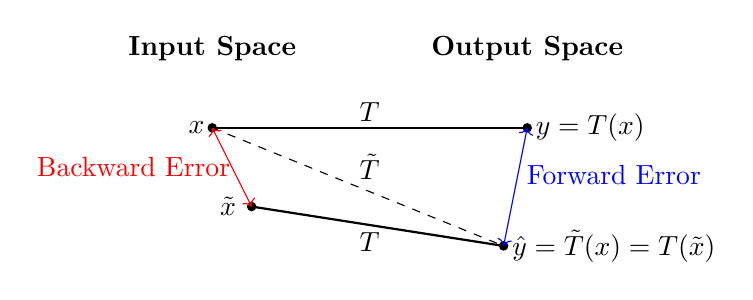
\begin{tikzpicture}[scale=1]
        \draw (-2, 2) node {\bf{Input Space}};
        \draw (2, 2) node {\bf{Output Space}};
        \filldraw[fill=black] (-2, 1) circle (1.5pt);
        \draw (-2.2, 1) node {$ x $};
        \filldraw[fill=black] (-1.5, 0) circle (1.5pt);
        \draw (-1.8, 0) node {$ \tilde{x} $};
        \filldraw[fill=black] (2, 1) circle (1.5pt);
        \draw (2.8, 1) node {$ y=T(x) $};
        \filldraw[fill=black] (1.7, -0.5) circle (1.5pt);
        \draw (3.1, -0.5) node {$ \hat{y}=\tilde{T}(x)=T(\tilde{x}) $};
        \draw[thick] (-2, 1) -- (2, 1);
        \draw (0, 1.2) node {$ T $};
        \draw[thick] (-1.5, 0) -- (1.7, -0.5);
        \draw (0, -0.45) node {$ T $};
        \draw[dashed] (-2, 1) -- (1.7, -0.5);
        \draw (0, 0.5) node {$ \tilde{T} $};
        \draw[<->,red] (-2, 1) -- (-1.5, 0);
        \draw (-3, 0.5) node {\textcolor{red}{Backward Error}};
        \draw[<->,blue] (2, 1) -- (1.7, -0.5);
        \draw (3.1, 0.4) node {\textcolor{blue}{Forward Error}};
    \end{tikzpicture}
    \caption{前向误差和后向误差,实线表示理论计算过程,虚线表示浮点计算过程}
    \label{Backward-Forward}
\end{figure}

对前向误差进行分析的需要是显然的,通常情况下我们甚至直接使用前向误差作为衡量一种算法关于某一具体问题优劣的指标,相比之下,后向误差分析的重要性往往被忽略了。后向误差分析的概念最早由James H. Wilkinson提出和使用,“for his research in numerical analysis to facilitate the use of the high-speed digital computer, having received special recognition for his work in computations in linear algebra and \underline{‘backward’ error analysis}”,他于1970年获得图灵奖。由于浮点计算不可避免地会引入舍入误差,这部分误差往往难以直接给出,我们需要一种方法来衡量这部分误差对最终结果的影响,后向误差分析提供了这样一种工具,它将经由包含舍入误差的浮点计算过程得到的计算值$ \tilde{T}(x) $等价于在一个被扰动后得到的新系统中准确计算得到的$ T(\tilde{x}) $,这一操作将舍入误差对结果的影响视作系统自身被扰动的结果。于是,我们可以通过研究系统在受到扰动时对应解的变化情况来刻画舍入误差的影响。另外,借助后向误差和系统自身的特性,前向误差可以被间接地分析。

如果某种算法用于某一问题对应的后向误差足够小,则称这种方法是\emph{后向稳定的}(Backward stable)。后向稳定是一个相当苛刻的条件,甚至一些简单的系统的很多算法都不是后向稳定的(例如计算$ \cos $大多数算法),通常我们说某一算法关于某具体问题是\emph{数值稳定的}(Numerical stable)是指该算法满足混合前后向稳定条件:
\begin{equation}
    \hat{y} + \Delta y = \tilde{y} = T(\tilde{x}) = T(x+\Delta x),\quad \| \Delta y \|\leqslant \epsilon \| y \| , \| \Delta x \|\leqslant \epsilon \| x \|
\end{equation}
满足这一条件的算法被称为是\emph{混合前后向稳定的}(Mixed forward-backward stable)。(注:这里的稳定性与微分方程数值解中的稳定性不是同一概念。)

\begin{figure}[htpb]
    \centering
    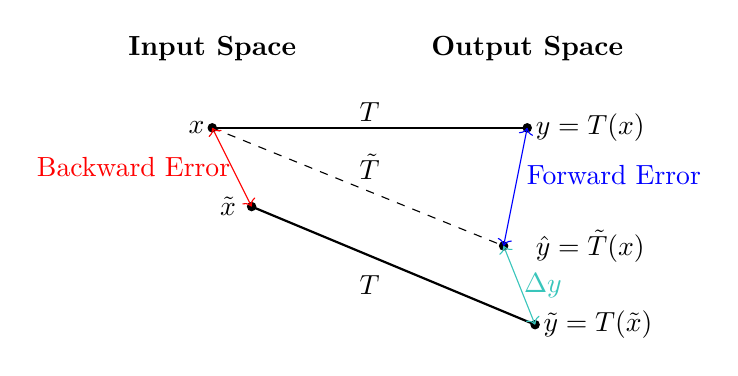
\begin{tikzpicture}[scale=1]
        \draw (-2, 2) node {\bf{Input Space}};
        \draw (2, 2) node {\bf{Output Space}};
        \filldraw[fill=black] (-2, 1) circle (1.5pt);
        \draw (-2.2, 1) node {$ x $};
        \filldraw[fill=black] (-1.5, 0) circle (1.5pt);
        \draw (-1.8, 0) node {$ \tilde{x} $};
        \filldraw[fill=black] (2, 1) circle (1.5pt);
        \draw (2.8, 1) node {$ y=T(x) $};
        \filldraw[fill=black] (1.7, -0.5) circle (1.5pt);
        \draw (2.8, -0.5) node {$ \hat{y}=\tilde{T}(x) $};
        \filldraw[fill=black] (2.1, -1.5) circle (1.5pt);
        \draw (2.9, -1.5) node {$ \tilde{y} = T(\tilde{x}) $};
        \draw[thick] (-2, 1) -- (2, 1);
        \draw (0, 1.2) node {$ T $};
        \draw[thick] (-1.5, 0) -- (2.1, -1.5);
        \draw (0, -1) node {$ T $};
        \draw[dashed] (-2, 1) -- (1.7, -0.5);
        \draw (0, 0.5) node {$ \tilde{T} $};
        \draw[<->,red] (-2, 1) -- (-1.5, 0);
        \draw (-3, 0.5) node {\textcolor{red}{Backward Error}};
        \draw[<->,blue] (2, 1) -- (1.7, -0.5);
        \draw (3.1, 0.4) node {\textcolor{blue}{Forward Error}};
        \draw[<->,miku] (1.7, -0.5) -- (2.1, -1.5);
        \draw (2.2, -1) node {\textcolor{miku}{$ \Delta y $}};
    \end{tikzpicture}
    \caption{混合前后向误差,实线表示理论计算过程,虚线表示浮点计算过程}
    \label{MixBackward-Forward}
\end{figure}

\subsubsection{内积,外积以及矩阵乘法}
我们以内积,外积以及矩阵乘法为例,简要介绍前向误差和后向误差的分析方法。

给定$ \bm{x} = (x_1,x_2,\cdots ,x_{n})^T $和$ \bm{y} = (y_1, y_2, \cdots, y_{n})^T $,则它们的内积和外积分别为
\[
    \bm{x}^T\bm{y} = \sum_{i=1}^{n}x_iy_i,\quad 
    \bm{x}\bm{y}^T = \begin{pmatrix}
        x_1y_1 & x_1y_2 & \cdots & x_1y_n \\
        x_2y_1 & x_2y_2 & \cdots & x_2y_n \\
        \vdots & \vdots & \ddots & \vdots \\
        x_ny_1 & x_ny_2 & \cdots & x_ny_n  
    \end{pmatrix}.
\]
首先考虑内积的数值计算,记$ s_j = \sum_{i=1}^j x_{i} y_{i} $为前$ j $项和,则我们有如下迭代关系
\[
    \hat{s}_j = fl(\hat{s}_{j-1} + fl(x_{j} y_{j})) = (\hat{s}_{j-1} + x_{j}y_{j}(1+\delta_j^{(1)}))(1+\delta_j^{(2)}),
\]
其中$ |\delta_j^{\ell}|\leqslant u $,因此
\[
    \begin{aligned}
        \hat{s}_n
        &= x_1y_1(1+\delta_1^{(1)})\prod_{i=2}^n(1+\delta_i^{(2)}) + x_2y_2(1+\delta_2^{(1)})\prod_{i=2}^n(1+\delta_i^{(2)})\\
        &+ x_3y_3(1+\delta_3^{(1)})\prod_{i=3}^n(1+\delta_i^{(2)}) + \cdots + x_ny_n(1+\delta_n^{(1)})(1+\delta_n^{(2)}).
    \end{aligned}
\]
由于所有的$ \delta_j^{(i)} $都满足相同的限制:$ |\delta_j^{(i)}|\leqslant u $,在这一简单情形下我们可以忽略这些量的区别,将它们统一记作$ \delta $,此时上式变为
\[
    \hat{s}_n = x_1y_1(1+\delta)^n + x_2y_2(1+\delta)^n + x_3y_3(1+\delta)^{n-1}+\cdots +x_ny_n(1+\delta)^2
\]

由于类似$ (1+\delta_i)^k $的量频繁地出现在误差分析过程中,而在其他应用场景为了更加细致的分析往往会保留角标,区分各个$ \delta_i $,这为误差分析带来了一些困难。我们现在给出如下非常实用的引理,它可以帮助我们漂亮地表示前向误差和后向误差。
\begin{lemma}\label{lem_1}
    给定$ |\delta_i|\leqslant u $,$ \rho_i=\pm 1 $($ i=1,2,\cdots ,n $),并且$ nu<1 $,则
    \begin{equation}
        \prod_{i=1}^n (1+\delta_i)^{\rho_i} = 1+\theta_n,
    \end{equation}
    其中
    \begin{equation}
        |\theta_n|\leqslant \frac{n u}{1 - n u}=:\gamma_n.
    \end{equation}
\end{lemma}

使用上述引理可以得到
\begin{equation}
    \hat{s}_n = x_1y_1(1+\theta_n) + x_2y_2(1+\theta_n) + \cdots + x_n y_n (1+\theta_2) = \bm{x}^T (\bm{y}+\Delta\bm{y})
\end{equation}
其中$ \Delta\bm{y} = (\theta_n y_1, \theta_n y_2, \cdots , \theta_2 y_n) $就是这一计算过程的后向误差,它满足
\[
    |\Delta \bm{y}| \leqslant \gamma_n |\bm{y}|
\]
这一事实表明这种内积计算方法是后向稳定的。这里的绝对值符号的作用是对其中各个分量取绝对值,即$ |\bm{y}| = (|y_1|,\cdots ,|y_n|)^T $。另一方面,前向误差为$ |\hat{s}_n-s_n| \leqslant \gamma_n \sum |x_iy_i| = \gamma |\bm{x}|^T |\bm{y}| $。仅根据这一估计无法判断是否前向稳定,在一些特别情况下,例如当$ \bm{x}=\bm{y} $时,前向稳定是显然的。像这样难以直接分析前向稳定性时,我们可以借助后向误差分析来刻画前向误差,一般地,我们有
\begin{equation}
    \text{Forward Error} \lesssim \text{Condition Number} \times \text{Backward Error}
\end{equation}
其中条件数刻画了计算结果对于输入的敏感性,在下一节我们将详细讨论条件数的概念,在这一例子中,我们固定$ \bm{x} $视作参数,以$ \bm{y} $作为变量,于是条件数为
\[
    \kappa = \frac{DT(x)\cdot x}{T(x)} = \frac{(\bm{x}, \bm{y})}{\bm{x}^T\bm{y}}=1
\]
因此前向误差可以被后向误差控制,这表明该计算也是前向稳定的。

另外,使用一些技巧可以降低后向误差估计中的系数$ \gamma_n $。当$ n=2^k $时,类似于二分排序的想法,可以采用分而治之(Divide and Rule)的思想将原本的求和分为两个较小的求和,每一部分对$ 2^{k-1} $个分量积进行求和,在对这两个较小的求和重复这样的操作直到对无需进行求和只需做一次分积。不难猜到,这一操作可以将该系数降低到$ \gamma_{\lceil \log_2 n \rceil + 1} $。

下面考虑外积$ A=\bm{x} \bm{y}^T $,类似地有
\[
    \hat{A} = \begin{pmatrix}
        x_1y_1(1+\theta_{11}) & x_1y_2(1+\theta_{12}) & \cdots & x_1y_n(1+\theta_{1n}) \\
        x_2y_1(1+\theta_{21}) & x_2y_2(1+\theta_{22}) & \cdots & x_2y_n(1+\theta_{2n}) \\
        \vdots & \vdots & \ddots & \vdots \\
        x_ny_1(1+\theta_{n1}) & x_ny_2(1+\theta_{n2}) & \cdots & x_ny_n(1+\theta_{nn}) 
    \end{pmatrix} = A+\Delta A
\]
其中$ |\Delta A|\leqslant u |A| $,此即前向误差估计。然而,由于$ \hat{A} $通常不是秩一矩阵,因此$ \hat{A} $无法写成$ (\bm{x}+\Delta \bm{x})(\bm{y}+\Delta \bm{y})^T $的形式,这暗示了外积计算通常不是后向稳定的。

内积和外积计算在后向稳定性上的不同其实是一个更一般的原则的特例:通常来说,相比于输出空间的维数大于输入空间维数的计算过程,输出空间维数小于输入空间维数的计算过程更容易是后向稳定的。

最后考虑矩阵乘法的数值计算,首先考虑矩阵-向量积$ \bm{y} = A \bm{x} $,其中$ A=(\bm{a}_1, \bm{a}_2, \cdots , \bm{a}_m)^T $是$ m\times n $阶矩阵。根据矩阵乘法的定义,$ y_i = \bm{a}_i^T \bm{x} $是一个内积,根据之前的结果
\[
    \hat{y}_i = (\bm{a}_i + \Delta \bm{a}_i)^T \bm{x}, \quad |\Delta \bm{a}_i|\leqslant \gamma_n |\bm{a}_i| 
\]
于是
\[
    \hat{\bm{y}} = (A + \Delta A)\bm{x}, \quad |\Delta A|\leqslant \gamma_n |A|
\]
其中$ \Delta A $为该计算过程的后向误差,同时可以得到前向误差估计
\[
    |\hat{\bm{y}} - \bm{y}| \leqslant \gamma_n |A| |\bm{x}|
\]
接下来考虑矩阵-矩阵积$ C=AB $,与矩阵-向量积类似,我们有
\[
    \hat{c}_{ij} = (\bm{a}_i + \Delta \bm{a}_i^{(j)})^T \bm{b}_j, \quad |\Delta \bm{a}_i^{(j)}|\leqslant \gamma_n |\bm{a}_i|.
\]
于是$ \hat{\bm{c}}_j = (A+\Delta A^{(j)})\bm{b}_j $,进而
\[
    \hat{C} = ((A + \Delta A^{(1)})\bm{b}_1, (A + \Delta A^{(2)})\bm{b}_2, \cdots , (A + \Delta A^{(n)})\bm{b}_n),
\]
可见$ C $的每列都具有一个很小的后向误差,因此每一列的计算都是后向稳定的,但是关于$ C $整体的后向误差估计是比较困难的。同样地我们可以有前向误差估计
\[
    |\hat{C}-C|\leqslant \gamma_n |A||B|.
\]
这一估计与理想的$ |\hat{C}-C|\leqslant \gamma_n |AB| $(前向稳定)有一些区别,但上式是我们所能期望的最好结果,因为确实存在矩阵$ A,B $以及$ |\Delta A|\leqslant \gamma |A| $满足
\[
    |\hat{C}-C|_{ij} = |\Delta A\cdot B|_{ij}= \gamma (|A| |B|)_{ij}> \gamma |AB|_{ij},
\]
这一事实反映了线性系统在受到相对扰动时的敏感性。

这一小节的最后,我们给出引理\ref{lem_1}的矩阵形式推广,当使用不同的范数时估计的形式都完全类似,这些结果在与矩阵有关的误差分析里可能会有用:
\begin{lemma}
    给定$ X_j+\Delta X_j\in \mathbb{R}^{n\times n} $:
    \begin{itemize}
        \item 如果$ \| \Delta X_j \| \leqslant \delta_j \| X_j \| $,其中$ j=1,2,\cdots, m $,$ \| \cdot \| $是相容范数($ \| AB \|\leqslant \| A \|\| B \| $),则
        \begin{equation}
            \| \prod_{j=1}^m (X_j +\Delta X_j)-\prod_{j=1}^m X_j \| \leqslant \left[ \prod_{j=1}^m(1+\delta_j)-1 \right] \prod_{j=1}^m \| X_j \|,
        \end{equation}
        \item 如果$ \| \Delta X_j \|_F \leqslant \delta_j \| X_j \|_2 $,其中$ j=1,2,\cdots, m $,$ \| \cdot \|_F $是Frobenius范数(元素平方和开方),$ \| \cdot \|_2 $是矩阵2范数(最大奇异值),则
        \begin{equation}
            \| \prod_{j=1}^m (X_j +\Delta X_j)-\prod_{j=1}^m X_j \|_{F} \leqslant \left[ \prod_{j=1}^m(1+\delta_j)-1 \right] \prod_{j=1}^m \| X_j \|_2,
        \end{equation}
        \item 如果$ | \Delta X_j | \leqslant \delta_j | X_j | $,其中$ j=1,2,\cdots, m $,则
        \begin{equation}
            | \prod_{j=1}^m (X_j +\Delta X_j)-\prod_{j=1}^m X_j | \leqslant \left[ \prod_{j=1}^m(1+\delta_j)-1 \right] \prod_{j=1}^m | X_j |.
        \end{equation}
    \end{itemize}
\end{lemma}

\subsection{基础数值计算}
这一节总结了一些在数值计算中常用的基础计算,包括求和,多项式计算,以及有理函数计算。
\subsubsection{求和}
计算机借助浮点计算可以快速高效地完成巨量的运算,但实际上哪怕是最简单的求和运算,浮点运算引入的误差也可能对结果造成致命的影响,在不同的情形下我们需要选取不同的求和方法。在计算机上进行求和时,按照不同的顺序求和时得到的结果都往往会不同。

常见的对$ n $个数进行求和$ \sum_{i=1}^n x_i $的方法有如下三种:
\begin{enumerate}
    \item 迭代求和(recursive summation):直接按照顺序进行求和。
    \begin{verbatim}
        s = 0
        for i = 1 to n
            s = s + x_i
    \end{verbatim}
    \item 分片求和(pairwise summation):使用分而治之法,分$ \lceil \log_2 n\rceil $个阶段求和。这种方法可以并行计算。
    \begin{figure}[htpb]
        \centering
        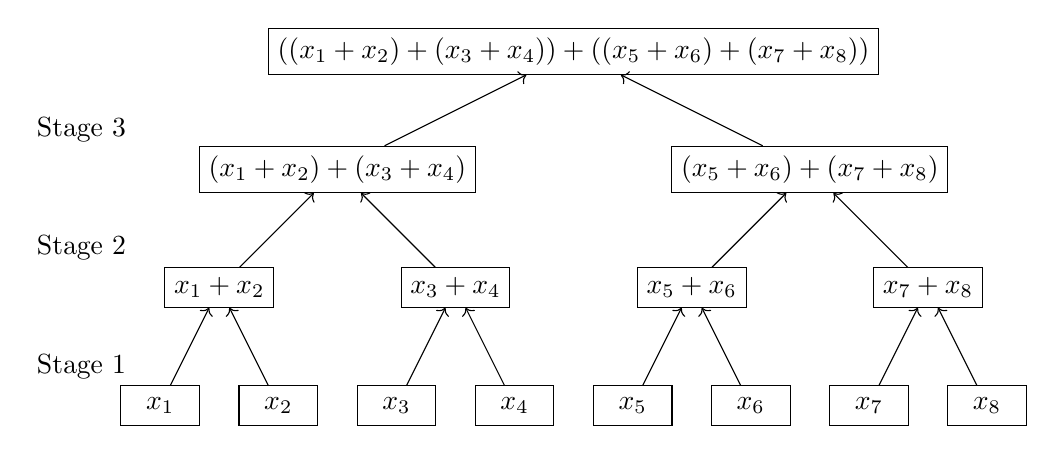
\begin{tikzpicture}[node distance=1.5cm, every node/.style={draw, rectangle, minimum height=0.5cm, minimum width=1cm}]
            % Level 1
            \node (a1) at (0,0) {$ x_1 $};
            \node (a2) [right of=a1] {$ x_2 $};
            \node (a3) [right of=a2] {$ x_3 $};
            \node (a4) [right of=a3] {$ x_4 $};
            \node (a5) [right of=a4] {$ x_5 $};
            \node (a6) [right of=a5] {$ x_6 $};
            \node (a7) [right of=a6] {$ x_7 $};
            \node (a8) [right of=a7] {$ x_8 $};
        
            % Level 2
            \node (b1) [above of=a1, xshift=0.75cm] {$ x_1+x_2 $};
            \node (b2) [above of=a3, xshift=0.75cm] {$ x_3+x_4 $};
            \node (b3) [above of=a5, xshift=0.75cm] {$ x_5+x_6 $};
            \node (b4) [above of=a7, xshift=0.75cm] {$ x_7+x_8 $};
        
            % Level 3
            \node (c1) [above of=b1, xshift=1.5cm] {$ (x_1+x_2)+(x_3+x_4) $};
            \node (c2) [above of=b3, xshift=1.5cm] {$ (x_5+x_6)+(x_7+x_8) $};
        
            % Level 4
            \node (d1) [above of=c1, xshift=3cm] {$ ((x_1+x_2)+(x_3+x_4))+((x_5+x_6)+(x_7+x_8)) $};
        
            % Edges
            \draw[->] (a1) -- (b1);
            \draw[->] (a2) -- (b1);
            \draw[->] (a3) -- (b2);
            \draw[->] (a4) -- (b2);
            \draw[->] (a5) -- (b3);
            \draw[->] (a6) -- (b3);
            \draw[->] (a7) -- (b4);
            \draw[->] (a8) -- (b4);
        
            \draw[->] (b1) -- (c1);
            \draw[->] (b2) -- (c1);
            \draw[->] (b3) -- (c2);
            \draw[->] (b4) -- (c2);
        
            \draw[->] (c1) -- (d1);
            \draw[->] (c2) -- (d1);

            \node[draw=none] (stage1) at (-1,0.5) {Stage 1};
            \node[draw=none] (stage2) at (-1,2) {Stage 2};
            \node[draw=none] (stage3) at (-1,3.5) {Stage 3};
        \end{tikzpicture}
        \caption{对8个数字进行分片求和的过程(二叉树)}
    \end{figure}
    \item 插入求和(insertion summation):边排序边求和,每做一次加法后将结果插入到合适的位置以保持序列的单调性,例如
    \[
        (2,4,5,1)\to (1,2,4,5)\to (3,4,5)\to (5,7) \to 12.
    \]
\end{enumerate}

\iffalse
\begin{algorithm}
    \caption{Variable Step Method by Pade\&Anti-Pade Method}
    \KwData{IVP:$y' = F(t, y),y(t_0) = y_0,t_0,T,h_{min},h_{max}$}
    \KwResult{Numerical Solution of IVP in $[t_0, T]$}
    Initialization: $t(1) = t_0, y(1) = y_0, h = h_{max}, i = 1, \ell = 0.5$\;
    \While{$t \leq T$}{
        Calculate Taylor coefficients of solution at $t$ by Taylor Method\;
        Construct $(m/n)_f$ and $[[m/n]]_f$ at $t=t(i)$\;
        Estimate Error:\ $ \hat{e} = |(m/n)_f - [[m/n]]_f| /2$\;
        \If{$\hat{e}(h) \leq tol$}{
            $t(i+1) = t(i) + h, y(i+1) = (m/n)_f(h)$\;
        }
        \Else{
            Update step size:\ $h = \ell h(tol / \hat{e}(h))^{1/(m+n+1)} $\;
            \If{$h < h_{min}$}{
                $h = h_{min}$\;
            }
            $t(i+1) = t(i) + h, y(i+1) = (m/n)_f(h)$\;
        }
        $i = i + 1$\;
    }
    \Return $(t, y)$\;
\end{algorithm}
\fi


上述三种算法均可以视作算法\ref{alg:sum}的特例,分析算法\ref{alg:sum}可以看出,不管使用那种形式的算法,都需要$ n-1 $次加法运算,即循环次数为$ n-1 $,如果记第$ i $次加法计算为$ T_i = x_i^{(1)} + y_i^{(1)} $,则根据浮点计算的性质
\[
    \hat{T}_i = \frac{x_i^{(1)} + y_i^{(1)}}{1+\delta_i},\quad |\delta_i|\leqslant u, i=1,2,\cdots, n-1.
\]
每一次加法都会引入一个局部误差$ \delta_i \hat{T}_i $,由于算法中各步都是线性的,于是使用归纳法可以得到总的前向误差为
\[
    E_n = S_n - \hat{S}_n = T_{n-1} - \hat{T}_{n-1} = \sum_{i=1}^{n-1} \delta_i \hat{T}_i.
\]
因此
\[
    |E_n| \leqslant u \sum_{i=1}^{n-1} |\hat{T}_i|,
\]
由于$ |\hat{T}_i|\leqslant \sum_{j=1}^n |x_j|+O(u) $,所以上式右侧可以进一步放宽为
\begin{equation}\label{eq:forward_error_sum}
    |E_n| \leqslant (n-1)u \sum_{j=1}^n |x_j|+O(u^2),
\end{equation}
这就是我们的前向误差估计。另一方面,由于在求和过程中,每一个元素最多经过了$ n-1 $次加法,因此在最终的计算结果中,每一个元素贡献的误差最多不超过$ \gamma_{n-1} $,因此按照算法\ref{alg:sum}进行的求和过程的后向误差估计可以写为
\begin{equation}\label{eq:backward_error_sum}
    \hat{S}_n = \sum_{i=1}^n x_i(1+\tau_i),\quad |\tau_i|\leqslant \gamma_{n-1}.
\end{equation}

\begin{algorithm}[htbp]
    \caption{基础求和算法}\label{alg:sum}
    \KwData{$ \mathcal{S} = \{x_1, x_2, \cdots, x_n \}.$}
    \KwResult{$ S_n = \sum_{i=1}^n x_i $}
    \While{$ \mathcal{S} $ contains more than one element}{
        Remove two numbers $ x $ and $ y $ from $ \mathcal{S} $\;
        Add their sum $ x+y $ to $ \mathcal{S} $\;
    }
    \Return the remaining element of $ \mathcal{S} $ as $ S_n $\;
\end{algorithm}

如果根据前向误差设计算法,那么就要最小化前向误差界中$ \sum_{i=1}^{n-1}|T_i| $,这涉及到对$ x_i $的排序,然而这一目标是相当难以达成的,可以证明为最小化这一误差界而对$ x_i $排序的问题是NP难的。但对于前面的几种求和方法,我们有一些足够好的策略使得前向误差界在一些情况下接近最小。

首先对于迭代求和,常用的有如下三种实现方式:
\begin{itemize}
    \item Psum:从$ \mathcal{S} $中最小的$ x_j $开始,在第$ i $次求和时,选取使$ |\hat{T}_i| = |\hat{S}_{i+1}| $最小的方式;
    \item 升序求和:先对$ \mathcal{S} $进行升序排序,再进行求和;
    \item 降序求和:先对$ \mathcal{S} $进行降序排序,再进行求和;
\end{itemize}
当$ \mathcal{S} $内各元素的符号相同时,升序求和的前向误差界在算法\ref{alg:sum}中各种算法中是最小的,在最小化前向误差的意义下是最优的。而当求和过程中出现了严重的相消现象,即$ |\sum_{i=1}^n x_i|\ll\sum_{i=1}^n |x_i| $时,则推荐使用降序求和,尽管这种情况下降序求和可能无法保证得到最优的前向误差界。至于当$ \mathcal{S} $中的元素符号混杂但又没有严重的相消现象时,Psum方法在实际操作中可能是三种方式中最好的选择。

对于分片求和,我们实际上有比(\ref{eq:forward_error_sum})和(\ref{eq:backward_error_sum})更加准确的前后向估计,例如当$ n=2^r $时,每个元素都经过了$ \log_2 n $次加法运算,所以我们可以将误差界中的常数项因子缩小到$ \gamma_{\log_2 n} $得到
\begin{equation}
    \hat{S}_n = \sum_{i=1}^n \left[ x_i\prod_{j=1}^{\log_2 n} (1+\delta_i^{(j)}) \right] ,\quad |\delta_i^{(j)}| \leqslant u,
\end{equation}
于是前向误差为
\begin{equation}
    |E_n| \leqslant \gamma_{\log_2 n} \sum_{i=1}^n |x_i|.
\end{equation}
在一般的情形下,$ \gamma_{\log_2 n} $已经是算法\ref{alg:sum}中各实现中所能期望的最小误差界系数。从这个角度来看,分片求和以牺牲内存为代价成功换取了高效的可并行计算性和准确的最终结果。

最后考虑插入求和,不难发现这种方法实际上就相当于尝试在第$ i $次求和时最小化$ |\hat{T}_i| $,当$ \mathcal{S} $中元素符号相同时,插入求和的前向误差界是算法\ref{alg:sum}的所有实例中最小的。

\paragraph*{补偿求和(Compensated Summation)}
之前的求和算法我们都只给出了先验的前后向误差估计,而利用实际计算中得到的中间结果,我们可以在计算过程中同时进行误差估计,当计算完成时误差估计也将完成,这种误差估计方式称为运行误差分析(Running Error Analysis),通常由于充分利用了计算的中间结果,运行误差估计得到的误差估计值会显著小于先验的误差估计界。更重要的是,在计算过程中进行误差估计有助于在下一步计算中调整计算策略,从而使得计算结果更加准确。将这一思想用于求和计算就得到了补偿求和算法。

补偿求和的基础是对浮点加法进行误差估计,例如在计算三个数$ x,y,z $的和时,记$ s=x+y $,则第一次求和满足如下关系:
\[
    \hat{s} + e = x+y
\]
我们需要在计算过程中估计$ e $,这样就可以在对$ x $和$ y $求和得到$ \hat{s} $之后,在要计算$ \hat{s}+z $时,以$ fl(\hat{s} +fl(z+\hat{e})) $作为最终的结果,其中的$ \hat{e} $就是该求和过程的一个补偿。需要指出的是这一计算的顺序的重要性,补偿$ \hat{e} $只在加在下一个元素$ z $上才有意义,因为$ \hat{s} $已经是$ x+y $的最优浮点表示了,即$ fl(\hat{s} + \hat{e}) = \hat{s} $是无效的操作。关于补偿$ e $的数值计算,Kahan给出了一种著名的估计方法,这种估计基于加法的无误差计算(Error-Free Computation)。给定两个准确的实数$ a $和$ b $满足$ |a|\geqslant |b| $,则求和误差满足
\begin{equation}
    e = -[((a+b)-a)-b] = (a-\hat{s})+b,
\end{equation}
并且在使用$ 2 $作为基数时,我们有
\begin{equation}
    \hat{s} + \hat{e} = x + y, 
\end{equation}
即$ \hat{e} $是真实误差$ e $的准确估计。以补偿求和方式计算的迭代求和算法如算法\ref{alg:compensated_sum}所示。图\ref{fig:EulerSum}展示了使用有无补偿的求和对单精度下的Euler法的影响,当计算步长$ h $较小时,有补偿的求和方法的误差界远小于没有补偿的求和方法的误差界,代码见附录\ref{code:EulerSum}。

\begin{figure}[htpb]
    \centering
    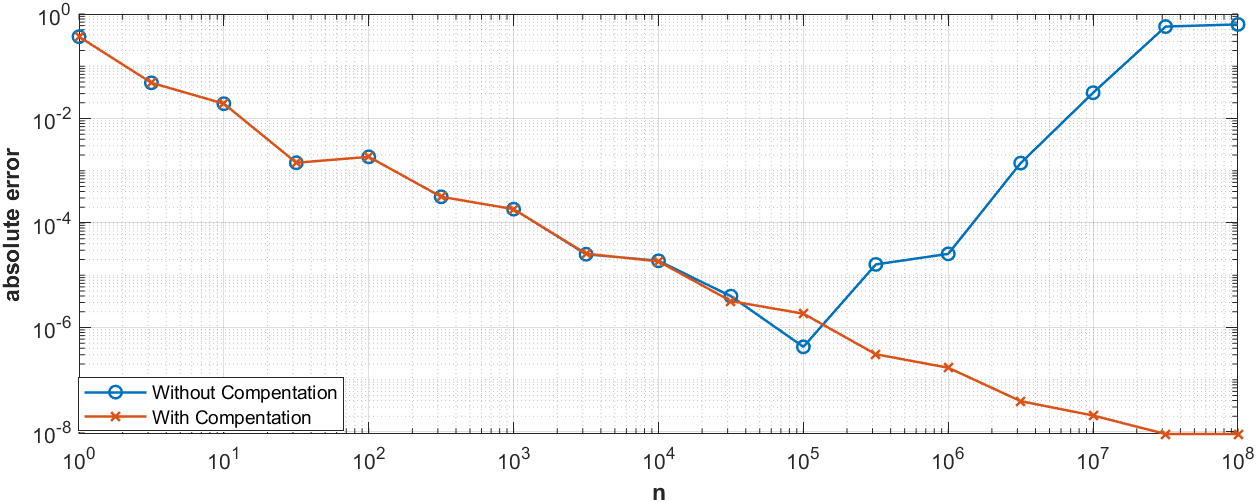
\includegraphics[width=0.6\textwidth]{EulerSum.png}
    \caption{单精度下分别使用有无补偿的Euler法求解$ [0,1] $上的初值问题$ y' = -y, y(0)=1 $得到的数值解在$ x=1 $处的绝对误差,其中计算步长为$ h = 1 / n $。}
    \label{fig:EulerSum}
\end{figure}

需要指出的是上述补偿方式并不是完美的:首先$ \hat{e} $本身的计算可能并不是准确的,因为相加的两个元素可能并不满足$ |a|\geqslant |b| $,其次在计算$ y+e $时也会引入新的误差。但通过这一操作我们确实可以大大减小误差界,可以证明对$ n $个数进行补偿求和的后向误差公式为
\begin{equation}
    \hat{S}_n = \sum_{i=1}^n (1+\mu_i)x_i,\quad |\mu_i|\leqslant 2u + O(nu^2),
\end{equation}
这一误差界通常远小于之前的没有补偿的求和方法的误差界。相应地,补偿求和的前向误差估计为
\begin{equation}
    |E_n|\leqslant (2u + O(nu^2))\sum_{i=1}^n |x_i|.
\end{equation}

上述两个缺陷可以通过双重补偿求和(Doubly Compensated Summation)来解决,这种算法可以用较低精度实现高精度计算。如算法\ref{alg:doubly_compensated_sum}所示,在这一算法中,首先需要对$ \mathcal{S} $中的元素按照绝对值大小进行排序以修复算法\ref{alg:compensated_sum}的第一个缺点,接着按照升序的顺序进行求和,其中不仅估计了每一次加法的误差,还估计了每一次补偿的误差,这修复了算法\ref{alg:compensated_sum}的第二个缺点,于是每一次循环我们进行了两次补偿。这一算法的前向误差估计在$ n\leqslant \beta^{t-3} $时为
\begin{equation}
    |s_n - \hat{s}_n |\leqslant 2u|s_n|,
\end{equation}
因此是前向稳定的,并且相对前向误差可以维持在机器误差级别,是非常精确的一种算法。

总的来说,可以根据以下原则挑选求和的方式:
\begin{enumerate}
    \item 精度优先:尝试在足够高的浮点精度下使用迭代求和或者使用双重补偿求和;
    \item 计算总量$ n $巨大:分片求和或者补偿求和;
    \item 符号一致:升序求和或者插入求和;
    \item 相消严重:尝试降序求和或者使用双重补偿求和。
\end{enumerate}

\begin{algorithm}[htbp]
    \caption{Compensated Summation}\label{alg:compensated_sum}
    \KwData{$ \mathcal{S} = \{x_1, x_2, \cdots, x_n \}.$}
    \KwResult{$ S_n = \sum_{i=1}^n x_i $}
    Initialization: $ s = 0, e=0 $\;
    \For{$ i=1:n $}{
        $ temp = s $\;
        $ y = x_i + e $\;
        $ s = temp + y $\;
        $ e = (temp - s) + y \quad$ \% Evaluate the error of this addition\;
    }
    \Return $ s $ as $ S_n $\;
\end{algorithm}

\begin{algorithm}[htbp]
    \caption{Doubly Compensated Summation}\label{alg:doubly_compensated_sum}
    \KwData{$ \mathcal{S} = \{x_1, x_2, \cdots, x_n \}.$}
    \KwResult{$ S_n = \sum_{i=1}^n x_i $}
    Initialization: Sort $ \mathcal{S} $ s.t. $ |x_1|\geqslant |x_2|\geqslant \cdots \geqslant |x_n| $, let $ s_1 = x_1, c_1=0 $\;
    \For{$ k=2:n $}{
        $ y_k = c_{k-1}+x_k $                   \tcc*[r]{First Compensation}
        $ u_k = x_k - (y_k - c_{k-1}) $         \tcc*[r]{Error of First Compensation}
        $ t_k = y_k + s_{k-1} $                 \tcc*[r]{$ k $th Addition}
        $ v_k = y_k - (t_k - s_{k-1}) $         \tcc*[r]{Error of $ k $th Addition}
        $ z_k = u_k + v_k $\;
        $ s_k = t_k + z_k $                     \tcc*[r]{Second Compensation}
        $ c_k = z_k - (s_k - t_k) $             \tcc*[r]{Error of Second Compensation}
    }
    \Return $ s_n $ as $ S_n $\;
\end{algorithm}

在附录中我们给出几种无误差计算的方法(算法\ref{alg:efc}),这些方法可以用于基础浮点运算的误差估计和精度提高。
这些无误差计算方法将在多项式和有理函数的数值计算中发挥作用。

\subsubsection{多项式}
多项式在数值计算中有着广泛的应用,例如在插值、逼近、微分方程数值解等问题中都会涉及到多项式的计算。最经典也是最常用的多项式计算算法是Horner法则(秦九韶算法),这一算法的基本思想是将多项式的计算转化为一系列的乘法和加法运算而不进行昂贵的指数运算,相比于直接使用幂运算和加法运算,使用Horner法则节省了一部分多余的乘法运算,从而提高了计算效率。为计算多项式
\[
    p(x) = a_0 + a_1x + a_2x^2 + \cdots + a_nx^n,
\]
的值,Horner算法的计算过程如算法\ref{alg:horner}所示。
\begin{algorithm}
    \caption{Horner's Method}\label{alg:horner}
    \KwData{Coefficients $ a_0, a_1, \cdots, a_n $, variable $ x $.}
    \KwResult{$ y = p(x) $.}
    $ q_n = a_n $\;
    \For{$ i=n-1:-1:0 $}{
        $ q_i = a_i + x q_{i+1}(x) $\;
    }
    \Return $ p(x) = q_0(x) $\;
\end{algorithm}

算法\ref{alg:horner}需要$ 2n $次浮点运算,其中包含$ n $次乘法和$ n $次加法,该算法等价于如下计算方式:
\[
    q_0 = a_0 + x(a_1 + x(a_2 + \cdots + x(a_{n-1} + x a_n)\cdots)).
\]

分析如上算法不难发现,与之前的内积计算类似,由归纳法可知使用Horner法计算多项式的后向误差满足
\begin{equation}
    \hat{q}_0 = (1+\theta_1)a_0 + (1+\theta_3)a_1x + \cdots + (1+\theta_{2n-1})a_{n-1}x^{n-1} + (1+\theta_{2n})a_n x^n,
\end{equation}
前向误差满足$ |\hat{q}_0-q_0|\leqslant \gamma_{2n} \sum_{i=0}^n |a_i x^i| $。因此Horner法具有较小的后向误差,使用这种方法数值计算多项式相当于在准确地计算该多项式的系数被轻微扰动后的值,具有后向稳定性,但前向误差可能会比后向误差大得多。由于先验前向误差界$ \gamma_{2n} \sum_{i=0}^n |a_i x^i| $实在不能令人满意,我们希望找到一种方法更好地估计前向误差,一种常用的方式是像求和一样使用运行误差分析,借助中间结果来估计误差。具体来说,在算法\ref{alg:horner}的第$ i $步计算$ q_i $时,如下关系成立:
\begin{equation}
    (1+\epsilon_i) \hat{q}_i = a_i + x \hat{q}_{i+1}(1+\delta_i),\quad |\delta_i|, |\epsilon_i| \leqslant u,
\end{equation}
现在记$ f_i $是这一步计算$ \hat{q}_i $的前向误差,即$ f_i = \hat{q}_i - q_i $,则根据上式有
\[
    f_i = xf_{i+1} + x \hat{q}_{i+1}\delta_i - \epsilon_i \hat{q}_i,
\]
其中$ f_n=0 $。由上式可以得到如下估计
\[
    |f_i| \leqslant |x| |f_{i+1}| + u(|x| |\hat{q}_{i+1}| + |\hat{q}_i|),
\]
做一些变形可得
\[
    \frac{|f_i| / u + |\hat{q}_i|}{2} \leqslant |x|\frac{|f_{i+1}| / u + |\hat{q}_{i+1}|}{2} + |\hat{q}_i|,
\]
根据上式右端可以得到一个递推关系
\begin{equation}
    \mu_i = |x| \mu_{i+1} + |\hat{q}_i|, 
\end{equation}
其中$ \mu_i=(|f_i| / u + |\hat{q}_i|) / 2 $并且$ \mu_n = |\hat{q}_n| / 2 $。随着计算推进,我们在计算$ q_i $之后计算出$ \mu_i $,当$ i=0 $时使用$ \mu_0 $可以得到一个更好的前向误差估计,具体的算法如算法\ref{alg:horner_runerror}所示,该算法需要$ 4n $次浮点运算,相比于算法\ref{alg:horner}增加了一倍的计算量,但是得到了更好的前向误差估计。
\begin{algorithm}
    \caption{Horner's Method with Running Error Analysis}\label{alg:horner_runerror}
    \KwData{Coefficients $ a_0, a_1, \cdots, a_n $, variable $ x $.}
    \KwResult{$ y $ and $ \mu $ s.t. $ |y-p(x)|\leqslant \mu $}
    Initialization: $ q_n = a_n, \mu_n = |a_n|/2 $\;
    \For{$ i=n-1:-1:0 $}{
        $ q_i = a_i + x q_{i+1} $\;
        $ \mu_i = |x| \mu_{i+1} + |q_i| $ \tcc*[c]{Running Error Analysis}
    }
    $ y = q_0 $, $ \mu = u(2\mu_0-|q_0|) $\;
    \Return $ y, \mu $\;
\end{algorithm}

与求和类似,多项式的计算也可以借助引入补偿或使用无误差计算的方式来提升精度,一种实现方式如算法\ref{alg:compensated_horner}所示,该算法来自Graillat,Langlois和Louvet。
\begin{algorithm}
    \caption{Compensated Horner's Method}\label{alg:compensated_horner}
    \KwData{Coefficients $ a_0, a_1, \cdots, a_n $, variable $ x $.}
    \KwResult{$ y $.}
    Initialization: $ q_n = a_n, r_n = 0 $\;
    \For{$ i=n-1:-1:0 $}{
       $ [p_i, \pi_i] = \texttt{TwoProduct}(q_{i+1}, x) $ \tcc*[r]{Error-free multiplication:$ xq_{i+1} = p_i + \pi_i $}
       $ [q_i, \sigma_i] = \texttt{TwoSum}(p_i, a_i) $ \tcc*[r]{Error-free addition:$ p_i+a_i = q_i + \sigma_i $}
       $ r_i = (\pi_i+\sigma_i) + r_{i+1}\times x $\;
    }
    $ y = q_0 + r_0 $\;
    \Return $ y $\;
\end{algorithm}

算法\ref{alg:compensated_horner}实际上计算了如下两个多项式作为原本数值计算的补偿:
\begin{equation}
    p_\pi = \sum_{i=0}^{n-1} \pi_i x^i,\quad p_\sigma = \sum_{i=0}^{n-1} \sigma_i x^i,
\end{equation}
借助无误差计算我们最终得到的是
\[
    y = q_0 + p_\pi(x) + p_\sigma(x),
\]
其中$ q_0 $是经典Horner法给出的计算值。可以证明算法\ref{alg:compensated_horner}的前向误差满足
\begin{equation}
    |p(x) - y| \leqslant  u|p(x)| + \gamma_{2n}^2 \tilde{p}(|x|),
\end{equation}
此处$ \tilde{p}(x) = |a_0| + |a_1|x + \cdots + |a_n| x^n $,借助条件数写成相对误差形式为
\begin{equation}
    \frac{|p(x) - y|}{|p(x)|} \leqslant u + \gamma_{2n}^2 {\rm cond}(p,x).
\end{equation}
作为对比,经典Horner法的前向相对误差满足
\begin{equation}
    \frac{|p(x) - y|}{|p(x)|} \leqslant \gamma_{2n} {\rm cond}(p,x).
\end{equation}
这两个估计中的条件数以如下方式定义
\[
    {\rm cond}(p,x) = \limsup_{\epsilon\to 0}\left\{ \frac{|p(x) - \hat{p}(x)|}{\epsilon|p(x)|}:|a_i-\hat{a}_i|\leqslant \epsilon |a_i| \right\}  = \frac{\sum_{i=0}^n |a_i x^i|}{|p(x)|} = \frac{\tilde{p}(|x|)}{|p(x)|}.
\]

我们以一个简单的样例展示引入补偿对精度的改善。考虑使用单精度浮点数计算$ p(x) = (x-2)^3 $的值,图\ref{fig:Horner}展示了使用Horner法和补偿Horner法在2附近的101个点处计算$ p(x) $的数值结果以及绝对误差。从图中可以看出,使用补偿Horner法计算的精度远高于使用Horner法。实现代码见附录\ref{code:Horner}。
\begin{figure}
    \centering
    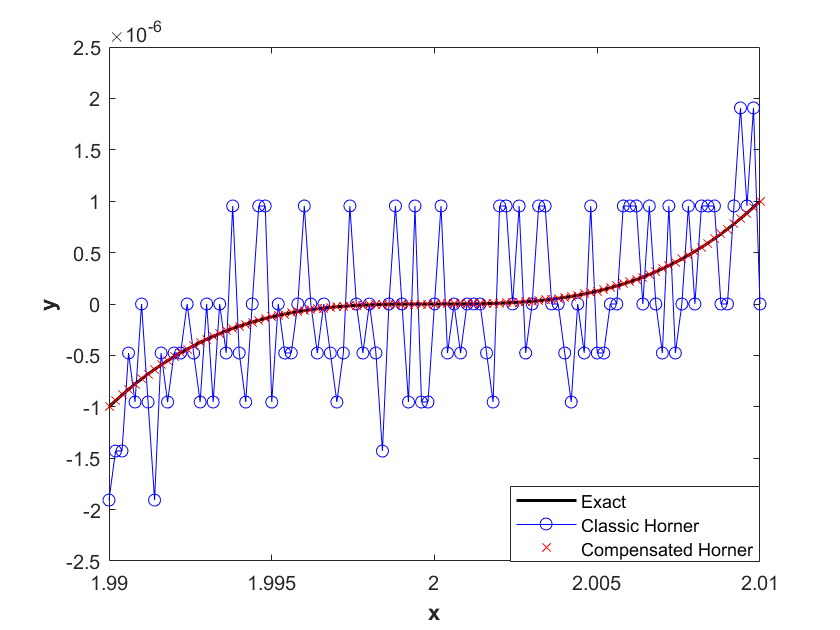
\includegraphics[width=0.4\textwidth]{polybyHorner.png}
    \hspace{1in}
    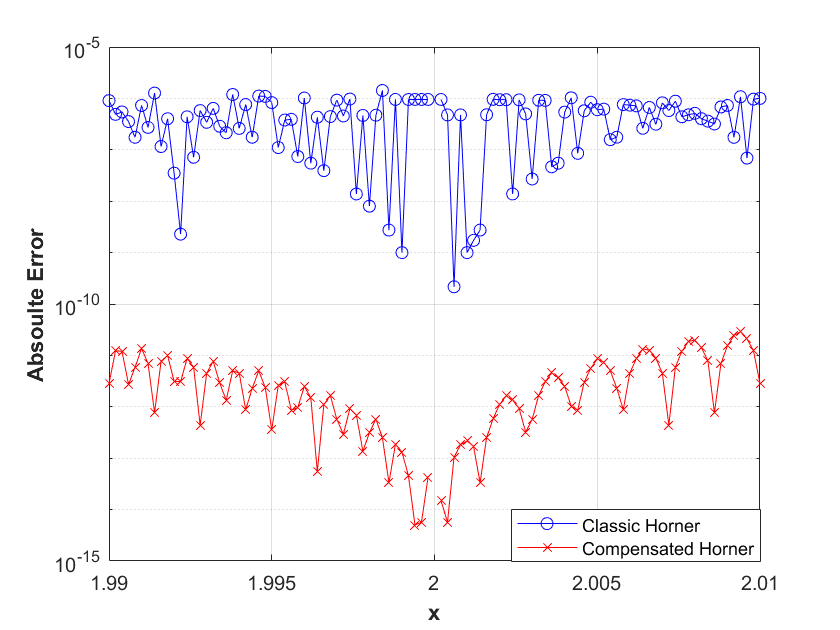
\includegraphics[width=0.4\textwidth]{ErrorbyHorner.png}
    \caption{单精度下使用Horner法和补偿Horner法计算$ p(x) = (x-2)^3 $的数值结果以及绝对误差}
    \label{fig:Horner}
\end{figure}

\subsubsection{有理函数}
有理函数的计算通常有两种方法,分别是基于多项式计算的算法\cite{graillat2018accurate}以及连分数算法。首先来考虑第一类算法,这是最符合直觉也最常用有理函数计算方式:先分别计算分母分子多项式再计算两者的商。根据上一小节的讨论,使用不同的多项式算法就会得到不同的有理函数计算算法。当使用经典的多项式计算算法时,可以证明计算有理函数
\[
    f(x) = \frac{p(x)}{q(x)}
\]
的前向误差满足
\begin{equation}
    \frac{|y - f(x)|}{|f(x)|} \leqslant u + [\gamma_{2n} + O(u^2)] {\rm cond}(f,x),
\end{equation}
该证明需要使用到$ {\rm cond}(f,x) = {\rm cond}(p,x) + {\rm cond}(q,x) $这一事实。而当使用补偿多项式计算算法时,可以证明前向误差满足
\begin{equation}
    \frac{|y - f(x)|}{|f(x)|} \leqslant 3u + O(u^2) + [2\gamma_{2n+1}^2 + O(u^3)] {\rm cond}(f,x),
\end{equation}
一个数值实例如图\ref{fig:RationalHorner}所示,该例子中我们通过调整分母多项式的阶数$ n $来控制条件数。
\begin{figure}[htpb]
    \centering
    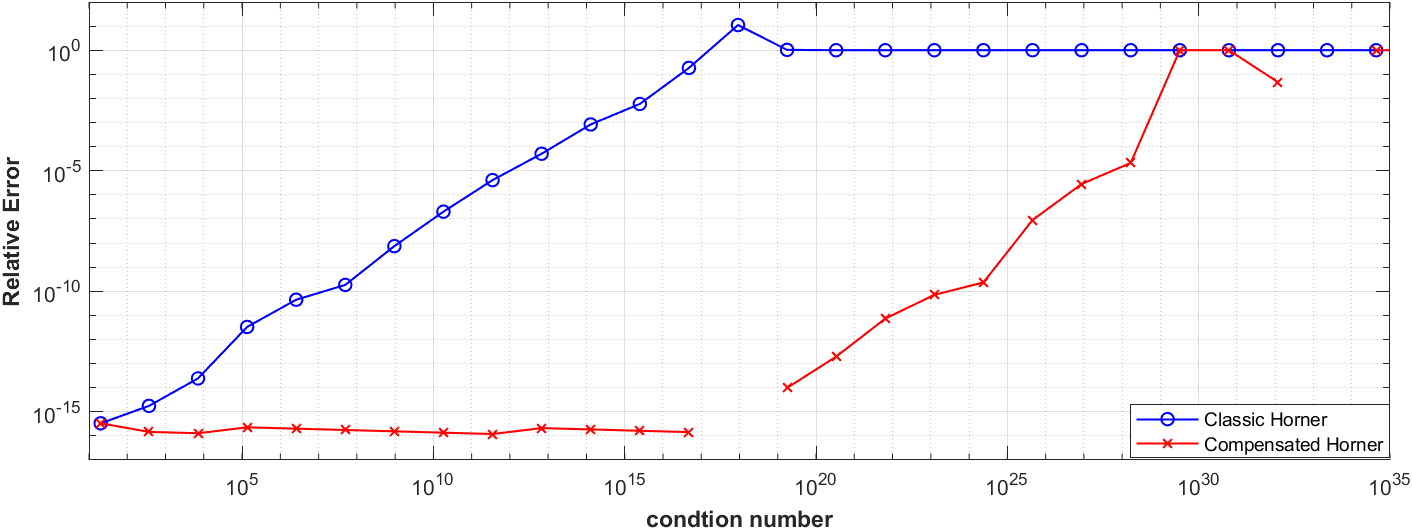
\includegraphics[width=0.8\textwidth]{RationalHorner.png}
    \caption{双精度下使用经典和补偿Horner法计算$ f(x) = (x+1)^3/(x-1)^n $在$ x=1.11 $处的值的相对误差,$ n=1,2,\cdots ,30 $,条件数$ {\rm cond}(f,x) = 1 + |x+1|^n / |x-1|^n $,缺失值下溢到0}
    \label{fig:RationalHorner}
\end{figure}

接下来考虑使用连分式形式计算有理函数,为此我们先考虑将分母分子都是幂级数的分式转化为连分式,这一方法被称为Viscovatov方法。直接计算可知形如
\[
    f(x) = \frac{d_{10} + d_{11} x + d_{12} x^2 + \cdots}{d_{00} + d_{01} x + d_{02} x^2 + \cdots},
\]
的函数在$ d_{10}\ne 0 $时可以被写为
\[
    \begin{aligned}
        f(x) = \frac{1}{\frac{d_{00}}{d_{10}} + \frac{d_{00} + d_{01} x + d_{02} x^2 + \cdots}{d_{10} + d_{11} x + d_{12} x^2 + \cdots} - \frac{d_{00}}{d_{10}}}
        &= \frac{d_{10}}{d_{00} + x\frac{(d_{01}d_{10} - d_{11}d_{00}) + (d_{02}d_{10}-d_{12}d_{00}) x + \cdots}{d_{10} + d_{11} x + d_{12} x^2 + \cdots}}\\
        &= \frac{d_{10}}{d_{00} + xf_1(x)}
    \end{aligned}
\]
其中$ f_1 $是一个新的与$ f $的形式相同的函数,它的分母级数是$ f $的分子级数,它的分子级数则可以通过$ f $的分子分母级数的系数计算得到,记为$ d_{20} + d_{21}x + d_{22}x^2 +\cdots  $,因此这一过程可以递推地进行下去,最终我们将得到如下形式的连分式
\begin{equation}
    f(x) = \cfrac{d_{10}}{d_{00} + 
    x\cfrac{d_{20}}{d_{10} + 
    x\cfrac{d_{30}}{d_{20}+ \cdots}}} = \polter{d_{10}}{d_{00}} + \polter{xd_{20}}{d_{10}} + \polter{xd_{30}}{d_{20}} + \cdots,
\end{equation}
其中
\begin{equation}
    d_{ij} = d_{i-1,0}d_{i-2,j+1} - d_{i-2,0}d_{i-1,j+1},\quad i\geqslant 2,j\geqslant 0.
\end{equation}
该计算可如下表示:
\[
    \begin{matrix}
        \vdots & \vdots & \vdots & \vdots & \\
        \textcolor{blue}{d_{i-2,0}} & \cdots & d_{i-2,j} & \textcolor{blue}{d_{i-2,j+1}} & \cdots \\
        \textcolor{blue}{d_{i-1,0}} & \cdots & d_{i-1,j} & \textcolor{blue}{d_{i-1,j+1}} & \cdots \\
        d_{i,0} & \cdots & \textcolor{red}{d_{i,j}} & d_{i,j+1} & \cdots \\
        \vdots & \vdots & \vdots & \vdots & 
    \end{matrix}
\]
如果将$ d_{ij} $排列成如上二维表,则计算顺序为从上向下。

\section{线性系统的微扰}
上一章中介绍了几种基础的数值计算,本章进一步考虑矩阵计算,通过研究线性系统在扰动下的表现,我们可以借助条件数来刻画浮点计算引入的舍入对数值计算的影响,并讨论数值稳定性和数值稳定算法的设计。准确的说,本章讨论的是线性系统$ Ax = b $在有解时,它的解$ x $在系统受到扰动,即$ A\to A+\Delta A, b\to b+\Delta b $时的变化情况。

\subsection{范数分析和分量分析}
当使用不同的方式刻画误差时,误差界的形式可能会有所不同,扰动分析也将具有不同的特点,通常我们使用范数或者绝对值两种方式来描述扰动和误差的大小,由此产生的分析方式和结果分别叫做范数分析和分量分析。使用范数和绝对值的区别主要在像空间不同:
\[
    \begin{aligned}
        \| \cdot \| : \mathbb{R}^n &\to \mathbb{R} \\
        \left\vert\ \cdot \ \right\vert : \mathbb{R}^n &\to \mathbb{R}^n_+
    \end{aligned}
\]
通常而言分量分析会比范数分析更加细致,可以让我们可以对每个分量的误差进行分析,但是相比于范数分析的简洁性,分量分析的结果可能更加复杂或者难以直接使用。
在本章中,我们使用$ E $来控制对$ A $的扰动,$ f $来控制对$ b $的扰动。

\subsubsection{范数分析}\label{sec:norm_analysis}
这一节我们使用范数来刻画扰动和误差。根据上一章的讨论,当使用浮点数计算$ Ax=b $得到的数值解$ \hat{x} $实际上可以视作扰动系统$ (A+\Delta A)y = b+\Delta b $的准确解,其中$ \Delta A $和$ \Delta b $是在浮点计算原系统时引入的后向误差,在本节我们使用范数研究这一后向误差。

首先我们从计算得到的数值解$ y=\hat{x} $出发。为了研究数值解$ y $所满足的系统究竟有多接近原来的系统,定义
\begin{equation}
    \eta_{E,f}(y) = \min_{\Delta A, \Delta b}\{ \epsilon: (A+\Delta A)y = b+\Delta b, \| \Delta A \|\leqslant \epsilon \| E \| , \| \Delta b \| \leqslant \epsilon \| f \| \},
\end{equation}
该量描述了为了让数值解$ y $满足扰动系统,我们需要最小对$ A $和$ b $引入多大的扰动,这反过来刻画了在数值计算过程中引入的后向误差大小。接着定义残差向量$ r = b - A y $,于是我们有
\[
    \Delta A y - \Delta b = r.
\]
根据范数的三角不等式以及相容性,我们有
\[
    \| r \| \leqslant \| \Delta A \| \| y \| + \| \Delta b \|,
\]
于是在$ \| \Delta A \|\leqslant \epsilon \| A \| , \| \Delta b \| \leqslant \epsilon \| f \| $时,我们有
\[
    \epsilon \geqslant \frac{\| r \|}{\| E \| \| y \| + \| f \|}.
\]
又因为当
\[
    \Delta A_{\min} = \frac{\| E \| \| y \|}{\| E \| \| y \| + \| f \| }rz^T, \quad \Delta b_{\min} = -\frac{\| f \|}{\| E \| \| y \| + \| f \| }r
\]
时$ \epsilon = \epsilon_{min} = \| r \|/(\| E \| \| y \| + \| f \|) $可以取到不等式的下界,其中$ z $是$ y $的对偶向量,满足
\[
    z^* y = \| z \|_D \| y \| = 1,\quad \text{where } \| x \|_D = \sup_{z\ne 0} \frac{|x^*z|}{\| z \| }.
\]
根据$ \eta_{E,f}(y) $的定义可得
\begin{equation}
    \eta_{E,f}(y) = \frac{\| r \|}{\| E \| \| y \| + \| f \|}.
\end{equation}
这一结果表明,当残差向量$ r $足够小时,数值解$ y $在后向误差意义下是一个良好的近似,这说明数值解的残差反映了数值解的准确程度。特别地,当$ E=A,f=b $时,$ \eta_{A,b}(y) $也被称作范数意义下的相对后向误差。

接下来考虑系统本身在受到的扰动对解的影响大小,即系统关于扰动的敏感性。考虑线性系统$ Ax=b $以及扰动系统$ (A+\Delta A)y = b + \Delta b $,其中$ \| \Delta A \| \leqslant \epsilon \| A \| $,$ \| \Delta b \| \leqslant \epsilon \| b \| $。因为当原系统有解,即$ A $可逆时,我们无法保证$ A+\Delta A $同样可逆,因此为了估计前向误差,需要尽量将$ A $和$ \Delta A $分开从而避免对$ A+\Delta A $求逆,为此我们结合$ Ax=b $和$ (A+\Delta A)y = b + \Delta b $得到
\[
    A(y-x) = \Delta b - \Delta A x + \Delta A (x-y),
\]
两侧左乘$ A^{-1} $可得
\[
    y-x = A^{-1}(\Delta b - \Delta A x + \Delta A (x-y)),
\]
于是
\[
    \| y-x \| \leqslant \| A^{-1} \| (\| \Delta b \| + \| \Delta A \| \| x \| + \| \Delta A \| \| x-y \|),  
\]
带入$ \| \Delta A \| \leqslant \epsilon \| A \| $,$ \| \Delta b \| \leqslant \epsilon \| b \| $整理可得前向误差估计
\begin{equation}\label{eq:normwise_forward_error}
    \frac{\| x-y \|}{\| x \| } \leqslant \frac{\epsilon}{1-\epsilon \| A^{-1} \| \| E \|} \left( \frac{\| A^{-1} \| \| f \|}{\| x \|} + \| A^{-1} \| \| E \| \right).
\end{equation}
该估计描述了系统受到扰动时解的相对变化幅度。可以证明前向相对误差可以达到上面估计右端关于$ \epsilon $同阶的程度,因此在$ \epsilon\to 0 $时上述估计是最优的。

\subsubsection{分量分析}\label{sec:component_analysis}
这一节我们再次考虑线性系统$ Ax=b $以及扰动系统$ (A+\Delta A)y = b + \Delta b $,但是使用绝对值代替范数来刻画扰动和误差。和之前一样,需要分别考虑后向误差和前向误差。

首先仍然从计算得到的数值解$ y=\hat{x} $出发,定义
\begin{equation}
    \omega_{E,f}(y) = \min_{\Delta A, \Delta b}\{ \epsilon: (A+\Delta A)y = b+\Delta b, | \Delta A | \leqslant \epsilon E , | \Delta b | \leqslant \epsilon f \},
\end{equation}
这个量的作用实际上与上一节中的$ \eta_{E,f}(y) $相同,只是使用了绝对值来刻画误差,同样定义残差向量$ r = b - A y $,与之前类似地可以证明分量意义下的后向误差为
\begin{equation}
    \omega_{E,f}(y) = \max_i \frac{| r_i |}{(E | y | + f)_i},
\end{equation}
当出现0做分母时,如果分子也为0则定义整体比值为0,否则定义为无穷。

接下来考虑系统本身在受到的扰动对解的影响大小。现在扰动的控制变为$ | \Delta A | \leqslant \epsilon E $,$ | \Delta b | \leqslant \epsilon f $,并且需要$ \epsilon\| |A^{-1}|E \|_\infty < 1 $,此时可以证明前向误差估计为
\begin{equation}\label{eq:componentwise_forward_error}
    \frac{\| x-y \|_\infty}{\| x \|_\infty} \leqslant \frac{\epsilon}{1-\epsilon \| |A^{-1}|E \|_\infty}  \frac{\| |A^{-1}|(E|x|+f) \|_\infty}{\| x \|_\infty }.
\end{equation}
同样地,前向相对误差可以达到上面估计右端关于$ \epsilon $同阶的程度。

从以上分析可知,除了系统本身,$ E $和$ f $的选取也会影响对前后向误差的估计,一般地,$ E $和$ f $有以下几种选择。
\begin{table}[h]
    \centering
    \begin{tabular}{ccc}
        \toprule
        Error & $ E $ & $ f $ \\
        \midrule
        relative & $ |A| $ & $ |b| $ \\
        row-wise & $ |A|ee^T $ & $ |b| $ \\
        columnwise & $ ee^T|A| $ & $ \| b \|_1 e $ \\
        normwise & $ \| A \|_\infty ee^T $ & $ \| b \|_\infty e $ \\
        \bottomrule
    \end{tabular}
    \caption{常用$ E,f $选取以及相应的误差}
    \label{tab:example}
\end{table}

\subsection{条件数}
这一小节介绍条件数,一般地,该量用于刻画系统的输出值关于输入值的敏感性。条件数高的问题被称为病态问题,条件数低的问题被称为良态问题。通常要得到病态问题在一定精度下的解要远远难于得到一个良态问题同一精度的解。正则化方法可以在一定程度上减轻问题的病态性。

条件数的一般性理论最早由Rice在1966年在文献\cite{rice1966theory}中给出。如今通常使用的条件数定义如下:
\begin{definition}
    给定某一问题$ f: \mathbb{R}^n \to \mathbb{R}^n$,它在某$ x $处的\href{https://nhigham.com/2020/03/19/what-is-a-condition-number/}{(相对)条件数}定义为
    \begin{equation}
        {\rm cond}(f,x) = \lim_{\epsilon\to 0^+} \sup_{\| \Delta x \|\leqslant \epsilon \| x \| }\frac{\| f(x+\Delta x) - f(x)\| }{\epsilon \| f(x) \| }.
    \end{equation}
\end{definition}
从以上定义来看,条件数是系统在受到某一量级的轻微扰动时输出值的最大相对变化幅度,正如之前所述,当扰动$ \Delta x $足够小时,我们有
\begin{equation}
    \frac{\| f(x+\Delta x) - f(x)\| }{\| f(x) \| }\lesssim {\rm cond}(f,x)\cdot \frac{\| \Delta x \|}{\| x \| },
\end{equation}
即
\begin{equation}
    \text{Forward relative error} \lesssim \text{Condition number} \times \text{Relative backward error}.
\end{equation}
其中的$ \lesssim $是指在$ \Delta x\to 0 $时不等关系成立。
需要注意定义中的$ x $并非系统的自变量,而是系统的一部分参数,例如考虑线性系统$ Ax=b $,这里的右端项$ b $实际上是上述定义中的$ x $,而问题的解$ x $是上述定义中的函数值$ f(x) $。

对于一些具体的问题,条件数可能有显式的表达式。
\begin{enumerate}
    \item 线性系统$ Ax = b $。当该系统有解,即$ A^{-1} $存在时,我们有$ f(b) = A^{-1}b $,于是
    \[
        {\rm cond}(A,b) = \lim_{\epsilon\to 0^+} \sup_{\| \Delta b \|\leqslant \epsilon \| b \| }\frac{\| A^{-1}\Delta b\| }{\epsilon \| A^{-1}b \| }
    \]
    其中
    \[
        \begin{aligned}
            \sup_{\| \Delta b \|\leqslant \epsilon \| b \| }\frac{\| A^{-1}\Delta b\| }{\epsilon \| A^{-1}b \| } \leqslant \frac{\| A^{-1} \Delta b^*\| }{\| A^{-1} b \| } \frac{\| b \|}{\| \Delta b^* \| } &= \frac{\| A^{-1} \Delta b^* \|}{\| \Delta b^* \| }\cdot \frac{\| Ax \|}{\| x \| }\\
            &\leqslant \| A^{-1} \| \| A \|,
        \end{aligned}
    \]
    因此线性系统的条件数具有一个与右端项$ b $无关而只与系数矩阵$ A $有关的上界(不是最优的),通常记$ \kappa(A) = \| A^{-1} \| \| A \| $,称为可逆矩阵$ A $的条件数。
    \item 计算标量函数$ f $。当$ f $在$ x $处可导时,我们有
    \[
        {\rm cond}(f,x) = \lim_{\epsilon\to 0^+} \sup_{|\Delta x|\leqslant \epsilon |x| }\frac{|f(x+\Delta x) - f(x)|}{\epsilon |f(x)|} = |x| \frac{|f'(x)|}{|f(x)|}.  
    \]
    \item 计算向量值函数$ f $。当$ f $在$ x $处的Jacobi矩阵$ J(x) $存在时,我们有
    \[
        {\rm cond}(f,x) = \lim_{\epsilon\to 0^+} \sup_{\| \Delta x \| \leqslant \epsilon \| x \| }\frac{\| f(x+\Delta x) - f(x) \|}{\epsilon \| f(x) \|} = \| x \| \frac{\| J(x) \|}{\| f(x)\| }.
    \]
\end{enumerate}
特别地,当在计算多项式$ p(x) = a_0 + a_1 x +\cdots+ a_n x^n $时,将系数向量$ a $视作输入,在无穷范数下我们有
\[
    {\rm cond}(p,a) = \frac{\max_i |a_i| \sum_{j=0}^n |x|^i}{x p'(x)}.
\]

另外,矩阵的条件数不仅取决于矩阵本身,同样也取决于所使用的范数:
\begin{enumerate}
    \item 使用$ L^2 $诱导范数时($ \| A \|_2 = \sqrt{\rho(A^*A)} = \sigma_{\max}(A) $,即谱范数),矩阵$ A $的条件数为
    \[
        \kappa(A) = \frac{\sigma_{\max}(A)}{\sigma_{\min}(A)},
    \]
    其中$ \sigma_{\max},\sigma_{\min} $分别是矩阵$ A $的绝对值最大和最小的奇异值。
    \item $ A $是正规矩阵时,$ A $的条件数为
    \[
        \kappa(A) = \frac{\lambda_{\max}(A)}{\lambda_{\min}(A)},
    \]
    其中$ \lambda_{\max},\lambda_{\min} $分别是绝对值最大和最小的特征值。
    \item $ A $是酉矩阵时,$ A $的条件数为$ \kappa(A)=1 $。
\end{enumerate}
我们要求在条件数的定义中使用的范数必须是一致的,即满足$ \| AB \| \leqslant \| A \| \cdot \| B \| $,在这种情况下注意到$ I = A^{-1}A $,并且$ \| I \| = 1 $,因此一般地
\begin{equation}
    \kappa(A) = \| A \| \cdot \| A^{-1} \|\geqslant 1.
\end{equation}
特别地,当使用Frobenius范数时($ \| A \|_F = \sqrt{\sum_{i,j}|a_{ij}|^2} = \sqrt{{\rm tr} (A^*A)} $, 或Euclidean范数),我们有更大的下界$ \kappa_F(A)\geqslant \sqrt{n} $($ n $是矩阵的行数或列数)。

自然地,当在原空间和像空间可以使用不同的范数时,我们使用由此诱导出的矩阵范数,于是条件数的定义可以推广到
\begin{equation}
    {\rm cond}(f,x) = \lim_{\epsilon\to 0^+} \sup_{\| \Delta x \|_1\leqslant \epsilon \| x \|_1 }\frac{\| f(x+\Delta x) - f(x)\|_2 }{\epsilon \| f(x) \|_2}.
\end{equation}
相应地,对于矩阵而言,如果$ A: (\mathbb{C}^n, \| \cdot \|_\alpha )\to (\mathbb{C}^n, \| \cdot \|_\beta ) $,记诱导得到的矩阵范数为$ \| A \|_{\alpha \beta} = \sup_{\| x \|_\alpha = 1 } \| Ax \|_\beta $,则
\begin{equation}
    \kappa_{\alpha \beta}(A) = \lim_{\epsilon\to 0^+} \sup_{\| \Delta A \|_{\alpha \beta}\leqslant \epsilon \| A \|_{\alpha \beta} }\frac{\| (A+A\Delta A)^{-1} - A^{-1} \|_{\beta \alpha} }{\epsilon \| A^{-1} \|_{\beta \alpha} }.
\end{equation}
在这种情况下我们仍然可以证明矩阵条件数具有与之前相同的形式(ASNA Th 6.4)
\begin{equation}
    \kappa_{\alpha \beta}(A) = \| A \|_{\alpha \beta} \| A^{-1} \|_{\beta \alpha}.
\end{equation}

除了之前提到的,条件数刻画了系统输出关于输入的敏感性,当问题是线性的时候,条件数也可以用来描述该系统距离奇异性的远近(ASNA Th 6.5, Gastinel, Kahan)
\begin{equation}
    {\rm dist}_{\alpha \beta}(A) = (\| A \|_{\alpha \beta} \| A^{-1} \|_{\beta \alpha})^{-1} = \kappa_{\alpha \beta}(A)^{-1},
\end{equation}
其中$ {\rm dist}_{\alpha \beta}(A) $是矩阵$ A $距离离它最近的奇异矩阵的相对距离,即
\begin{equation}
    {\rm dist}_{\alpha \beta}(A) = \min_{\Delta A} \left\{ \frac{\| \Delta A \|_{\alpha \beta}}{\| A \|_{\alpha \beta} }:A+\Delta A \text{ is singular.} \right\}  
\end{equation}

下面我们来进一步专门讨论线性系统$ Ax=b $的敏感性。在以上的分析中,根据条件数的定义,我们都只对右端项$ b $进行了扰动而假定系数矩阵$ A $是准确的,根据之前的讨论,使用浮点计算线性方程组时,舍入误差造成的影响相当于对$ A $进行了扰动,因此我们需要分析$ A $和$ b $同时受到扰动时的情况,为此让我们回到上一节的两种分析模式,由此可以给出相应的两个刻画这一敏感性的指标。
\subsubsection{范数意义下的条件数}
继续\ref{sec:norm_analysis}节的讨论,现以如下方式定义范数意义下的条件数。
\begin{definition}\bf{\textup{normwise condition number}}
    \begin{equation}
        \begin{aligned}
            \kappa_{E,f}(A,x) = \lim_{\epsilon\to 0^+} \sup_{\Delta A, \Delta b} \Big\lbrace \frac{\| \Delta x \|}{\epsilon \| x \|}: 
            &(A+\Delta A)(x+\Delta x) = b + \Delta b, \\
            &\| \Delta A \|\leqslant \epsilon\| E \|, \| \Delta b \| \leqslant \epsilon\| f \|  \Big\rbrace.
        \end{aligned}
    \end{equation}
\end{definition}
\noindent 在\ref{sec:norm_analysis}节中我们得到了前向误差估计(\ref{eq:normwise_forward_error}):
\begin{equation}
    \frac{\| \Delta x \|}{\| x \| } \leqslant \frac{\epsilon}{1-\epsilon \| A^{-1} \| \| E \|} \left( \frac{\| A^{-1} \| \| f \|}{\| x \|} + \| A^{-1} \| \| E \| \right),
\end{equation}
由于该估计在$ \epsilon\to 0 $时是最优的,因此
\begin{equation}
    \kappa_{E,f}(A,x) = \frac{\| A^{-1} \| \| f \|}{\| x \|} + \| A^{-1} \| \| E \| .
\end{equation}
特别地,当$ E=A,f=b $时,我们有
\[
    \kappa_{A,b}(A,x) = \frac{\| A^{-1} \| \| b \|}{\| x \|} + \| A^{-1} \| \| A \| = \| A^{-1} \| \| A \| \cdot \left( 1 + \frac{\| b \|}{\| A \| \| x \|} \right) = \kappa(A) \cdot \left( 1 + \frac{\| b \|}{\| A \| \| x \|} \right),
\]
所以$ \kappa(A)\leqslant \kappa_{A,b}(A,x)\leqslant 2\kappa(A) $,进而此时的前向误差估计可以被放宽为
\[
    \begin{aligned}
        \frac{\| \Delta x \|}{\| x \| } 
        \leqslant \frac{\epsilon}{1-\epsilon \| A^{-1} \| \| A \|} \left( \frac{\| A^{-1} \| \| b \|}{\| x \|} + \| A^{-1} \| \| A \| \right) 
        &= \frac{\epsilon \kappa_{A,b}(A,x)}{1-\epsilon \kappa(A)}\\
        &\leqslant \frac{2\epsilon \kappa(A)}{1-\epsilon \kappa(A)}.
    \end{aligned}
\]

尽管上述前向误差估计看上去既简单又容易操作,然而实际上该估计往往是非常宽松的,这一问题的主要原因是尽管$ \| \Delta A \|\leqslant \epsilon\| E \| $和$ \| \Delta b \| \leqslant \epsilon\| f \| $要求了扰动在范数意义下的相对大小足够小,但是对于$ A $和$ b $中那些较小的分量而言,扰动可能是相当大的。为了获得更细致的结果,我们需要使用分量分析。

\subsubsection{分量意义下的条件数}
这一节我们不再使用范数,而是使用绝对值,条件数的定义变为:
\begin{definition}\bf{\textup{componentwise condition number}}
    \begin{equation}
        \begin{aligned}
            {\rm cond}_{E,f}(A,x) = \lim_{\epsilon\to 0^+} \sup_{\Delta A, \Delta b} \Big\lbrace \frac{\| \Delta x \|_\infty}{\epsilon \| x \|_\infty}: 
            &(A+\Delta A)(x+\Delta x) = b + \Delta b, \\
            &| \Delta A |\leqslant \epsilon E , | \Delta b | \leqslant \epsilon f\Big\rbrace.
        \end{aligned}
    \end{equation}
\end{definition}
\noindent 在\ref{sec:component_analysis}节中我们得到了前向误差估计(\ref{eq:componentwise_forward_error}):
\begin{equation}
    \frac{\| \Delta x \|_\infty}{\| x \|_\infty} \leqslant \frac{\epsilon}{1-\epsilon \| |A^{-1}|E \|_\infty}  \frac{\| |A^{-1}|(E|x|+f) \|_\infty}{\| x \|_\infty },
\end{equation}
由于该估计在$ \epsilon\to 0 $时是最优的,因此
\begin{equation}
    {\rm cond}_{E,f}(A,x) = \frac{\| |A^{-1}|(E|x|+f) \|_\infty}{\| x \|_\infty }.
\end{equation}
另外,也可以定义矩阵$ A $的分量意义下的条件数为
\[
    {\rm cond}_{E,f}(A) = \sup_x {\rm cond}_{E,f}(A,x).
\]

特别地,当$ E=|A|,f=|b| $时,按照之前的定义
\[
    \begin{aligned}
        {\rm cond}_{|A|,|b|}(A,x) &= \frac{\| |A^{-1}|\cdot |A|\cdot|x| + |A^{-1}|\cdot |b| \|_\infty }{\| x \|_\infty },
    \end{aligned}
\]
因为上面的定义不仅与$ A,x $有关,还包含有$ b $,而实际上$ b $可以由$ A,x $确定,所以为了避免重复,在这种情况下我们往往使用另一种稍稍不同的定义,这种条件数被称作Skeel条件数[Skeel,1979]:
\begin{equation}
    {\rm cond}(A,x) = \frac{\| |A^{-1}| |A| |x| \|_\infty }{\| x \|_\infty },
\end{equation}
不难看出$ {\rm cond}_{|A|,|b|}(A,x) \leqslant {\rm cond}(A,x) \leqslant 2{\rm cond}_{|A|,|b|}(A,x) $。
相应的矩阵条件数为$ {\rm cond}(A) = {\rm cond}(A,e) = \| |A^{-1}||A| \|_\infty$,其中$ e = (1,1,\cdots ,1)^T $。

现在我们来建立两种条件数:$ {\rm cond} $和$ \kappa_\infty $之间的关系。首先,根据无穷范数的一致性
\[
    {\rm cond}(A) = \| |A^{-1}||A| \|_\infty\leqslant \| A^{-1} \|_\infty \| A \|_\infty  = \kappa_\infty(A),
\]
另一方面,注意到$ {\rm cond} $的一个重要性质是它在行放缩下是不变的,即对任意的对角阵$ D $,$ {\rm cond}(DA) = {\rm cond}(A) $,于是
\[
    \begin{aligned}
        {\rm cond}(A) = {\rm cond}(DA) = {\rm cond}(DA, e)
    \end{aligned}
\]
选取$ D = D_R $使得$ D_R|A|e = e $,注意到$ \| A \|_\infty = \| |A|e \|_\infty $,我们有
\[
    \begin{aligned}
        {\rm cond}(D_RA, e) = \| |A^{-1}D_R^{-1}| |D_RA|e \|_\infty 
        &= \| |A^{-1}D_R^{-1}|e \|_\infty \\
        &= \| A^{-1} D_R^{-1} \|_\infty \cdot 1\\
        &= \| A^{-1} D_R^{-1} \|_\infty \| D_RA \|_\infty = \kappa_\infty(D_RA) .
    \end{aligned}  
\]
其中第一行中的范数是向量范数,而后几行中的范数是矩阵范数,因此
\begin{equation}
    {\rm cond}(A) = \inf_D \kappa_\infty(DA), 
\end{equation}
并且当$ D = D_R $时有$ {\rm cond}(A) = \kappa_\infty(D_RA) $。进一步有[Chandrasekaran\&Ipsen,1995]
\[
    \frac{\kappa_\infty(A)}{\kappa_\infty(D_R)} \leqslant {\rm cond}(A)\leqslant \kappa_\infty(A)
\]
以及
\[
    \frac{\kappa_1(A)}{n\kappa_\infty(D_C)} \min_j \frac{\| A^{-1}e_j \|_\infty}{\| A^{-1} \|_1}\leqslant {\rm cond}(A,x) \leqslant \kappa_\infty(A).
\]
其中$ D_C $是满足$ e^T|A|D_C = e^T $的对角矩阵。从如上两个不等关系中可以看到,$ {\rm cond}(A) $只在矩阵$ A $各行的大小相差很大时才会远小于$ \kappa_\infty(A) $,类似地,$ {\rm cond}(A,x) $只在$ A $或者$ A^{-1} $的各列的大小相差很大时才会远小于$ \kappa_\infty(A) $。 

现在我们来总结一下这一节的各种条件数各自的作用:$ \kappa_\infty(A) $是范数意义下的矩阵条件数,它是系统条件数的一个上界,当它较大时,说明以$ A $作为系数矩阵的系统在最坏情形下可能会很敏感;$ {\rm cond}(A) $是分量意义下的矩阵条件数,当它较大时,说明线性系统$ Ax=b $在$ b $取\emph{某些}值时是比较敏感的; $ {\rm cond}(A,x) $是分量意义下的系统条件数,它刻画了某一\emph{确定}的系统$ Ax=b $在受到扰动时解的相对变化幅度(给定$ x $等价于给定右端项$ b $),当它较大时,说明该系统在受到相对扰动时是比较敏感的。需要注意的是,$ {\rm cond}(A) $较大时,$ {\rm cond}(A,x) $不一定较大,这种情况的出现表明尽管系统在某些右端项下是病态的,但是在右端项为$ b=Ax $时,系统在受到分量扰动时是良定的。例如考虑$ Ax=b $ [Kahan,1966],其中
\[
    A = 
    \begin{pmatrix}
        2 & -1 & 1\\
        -1 & \epsilon & \epsilon\\
        1 & \epsilon & \epsilon
    \end{pmatrix},\quad 
    x = 
    \begin{pmatrix}
        \epsilon\\
        -1\\
        1
    \end{pmatrix},\quad
    b = 
    \begin{pmatrix}
        2(1+\epsilon)\\
        -\epsilon\\
        \epsilon
    \end{pmatrix},
\]
计算可得$ \kappa_\infty(A) = 2(1+\epsilon^{-1}) $,$ {\rm cond}(A) = 3+(2\epsilon)^{-1} $,$ {\rm cond}(A,x) = 5 / 2+\epsilon $,这说明尽管$ A $是病态的,但是对于$ Ax=b $这一具体的特定问题,解在受到扰动时是比较稳定的。

通常来讲,分量分析给出的前向误差估计要比范数分析给出的更加精确,但一些情况下分量分析难以进行,需要根据具体问题选择合适的条件数进行分析。

\begin{table}[h]
    \centering
    \begin{tabular}{ccccc}
        \toprule
        Error & $ E $ & $ f $ & $ {\rm cond}_{E,f}(A,x) $ & $ {\rm cond}_{E,f}(A) $ \\
        \midrule
        relative & $ |A| $ & $ |b| $ & $ {\rm cond}(A,x) $ & $ {\rm cond}(A) $ \\
        row-wise & $ |A|ee^T $ & $ |b| $ & $ {\rm cond}(A,x) \frac{\| x \|_1}{\| x \|_\infty} $ & $ n {\rm cond}(A) $ \\
        columnwise & $ ee^T|A| $ & $ \| b \|_1 e $ & $ \| A^{-1} \|_\infty \frac{\| |A||x| \|_1}{\| x \|_\infty} $ & $ \kappa_\infty(A) $ \\
        normwise & $ \| A \|_\infty ee^T $ & $ \| b \|_\infty e $ & $ \kappa_\infty(A) $ & $ \kappa_\infty(A) $ \\
        \bottomrule
    \end{tabular}
    \caption{常用$ E,f $选取以及相应的条件数}
    \label{tab:cond}
\end{table}

最后,我们列举出一些关于条件数需要注意的事项,这些事实来自于Higham的博客\href{https://nhigham.com/2020/03/19/what-is-a-condition-number/}{What Is a Condition Number?}:
\begin{quote}
    \begin{itemize}
        \item 尽管条件数在一些情况下具有显式表达式,但是计算条件数往往和计算解一样昂贵,因此很多研究都尝试找到一种相对轻量的方法来估计条件数或给出某种条件数的上界。
        \item 虽然矩阵条件数$ \kappa(A)\geqslant 1 $,但是一般的条件数$ {\rm cond}(f,x) $不一定大于$ 1 $。
        \item 对于包括矩阵求逆、矩阵特征值和多项式根在内的一系列问题,可以证明相应的条件数是到最近奇异问题的相对距离的倒数。
        \item 由于条件数本身也是一个函数,所以一个自然的问题是:条件数的条件数是多少?对于包括前一点提到的那些问题在内的各种问题,条件数的条件数(近似)就是条件数。
    \end{itemize}
\end{quote}

\subsection{算法的数值稳定性}
图\ref{fig:stability}概括了四种数值稳定性的定义以及它们之间的关系。当换用不同的扰动上界时,可以得到不同的稳定性,例如按行意义下的后向稳定性(row-wise backward stability)是指算法满足$ \eta_{|A|ee^T,|b|}(\hat{x}) = O(u) $。
\begin{figure}[htpb]
    \centering
    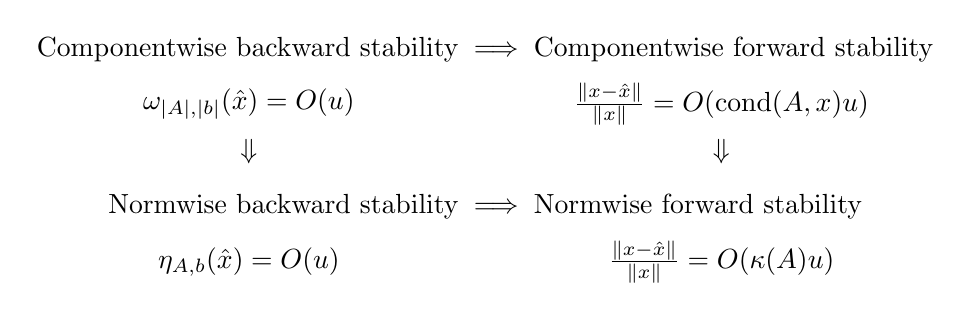
\begin{tikzpicture}
        \node at (0, 1.5) {$\text{Componentwise backward stability} \implies \text{Componentwise forward stability}$};
        \node at (-3, 0.8) {$\omega_{|A|,|b|}(\hat{x}) = O(u) $};
        \node at (3, 0.8) {$ \frac{\|x - \hat{x}\|}{\|x\|} = O(\text{cond}(A, x) u) $};
        \node at (0, -0.5) {$\text{Normwise backward stability} \implies \text{Normwise forward stability}$};
        \node at (-3, -1.2) {$\eta_{A,b}(\hat{x}) = O(u) $};
        \node at (3, -1.2) {$\frac{\|x - \hat{x}\|}{\|x\|} = O(\kappa(A) u) $};
        \node at (-3, 0.2) {$\Downarrow$};
        \node at (3, 0.2) {$\Downarrow$};
      \end{tikzpicture}
    \caption{后向稳定性和前向稳定性}
    \label{fig:stability}
\end{figure}

显然,对于线性系统而言,后向误差可以直接使用之前给出的公式进行计算:
\[
    \eta_{E,f}(\hat{x}) = \frac{\| r \|}{\| E \| \| \hat{x} \| +\| f \| },\quad
    \omega_{E,f}(\hat{x}) = \max_i \left[ \frac{|r_i|}{(E|\hat{x}|+f)_i} \right].
\]
这一方法的问题在于公式中的分母的计算值可能会发生下溢或出现零做除数,在系统是稀疏的情况下这尤其可能发生。LAPACK函数集(Linear Algebra PACKage,著名Fortran软件包)采用的策略是使用\verb|xyyRFS|例程,通过固定精度的迭代改进,尝试使$\omega_{|A|,|b|}\leqslant u$。如果分母的第$i$个分量小于$\text{safe\_min}/u$,则将$(n+1)\text{safe\_min}$加到分子和分母的第$i$个分量上。对于稀疏系统,有更复杂精巧的处理手段[Arioli\&Demmel\&Duff,1989]。

要估计前向误差,可以利用公式(\ref{eq:componentwise_forward_error}),借助条件数和后向误差来给出估计,不过由于真实解$ x $未知,因此需要使用近似解$ \hat{x} $来代替,这样就得到了前向误差的估计:
\begin{equation}
    \frac{\| x - \hat{x} \|_\infty}{\| \hat{x} \|_\infty} \leqslant \text{cond}_{E,f}(A,\hat{x})\cdot \omega_{E,f}(\hat{x}),
\end{equation}
或者使用公式(\ref{eq:normwise_forward_error}),得到
\begin{equation}
    \frac{\| x - \hat{x} \|}{\| \hat{x} \|} \leqslant \kappa_{E,f}(A,\hat{x})\cdot \eta_{E,f}(\hat{x}).
\end{equation}
由于$ E,f $的选取会影响到估计的效果,因此希望找到最合适的选择。实际上,根据$ r = b - A\hat{x} $,我们有
\[
    \frac{\| x-\hat{x} \|_\infty}{\| \hat{x} \|_\infty} = \frac{\| A^{-1}r \|_\infty}{\| \hat{x} \|_\infty}\leqslant \frac{\| |A^{-1}||r| \|_\infty}{\| \hat{x} \|_\infty}.
\]
上式中的不等号在$ A^{-1} $与$ b $的各元素符号相同时取等,因此该估计在不考虑符号时是最优的。之所以不选取$ \| A^{-1}r \|_\infty / \| \hat{x} \|_\infty $是因为由于使用浮点计算,无法得到$ r $和$ \| A^{-1}r \|_\infty $的准确值,实际上计算得到的是$ \hat{r} = fl(b-A \hat{x}) $,对这一计算结果我们有如下误差估计:
\[
    \hat{r} = r + \Delta r,\quad |\Delta r|\leqslant \gamma_{n+1}(|A| |\hat{x}| + |b|).
\]
因此需要使用$ |A^{-1}||r| $,所以实际中使用的是误差估计应为
\begin{equation}
    \frac{\| x-\hat{x} \|_\infty}{\| \hat{x} \|_\infty} \leqslant \frac{\| |A^{-1}|(|\hat{r}|+\gamma_{n+1}(|A||\hat{x}|+|b|)) \|_\infty}{\| \hat{x} \|_\infty}.
\end{equation}

\section{附录}

\hrule\vskip 1em
\paragraph*{Code 1:在Euler法求解$ y' = -y, y(0)=1 $中使用补偿求和}\label{code:EulerSum}
\begin{center}
    \hrule\vskip 0.5em
    \begin{verbatim}
        % y'=-y, y(0)=1, x\in [0,1]
        % Euler method
        
        function Euler_sum
        for r = 0:16
            n = 10^(r/2);
            e1(r+1) = classic(n) - exp(-1);
            e2(r+1) = compensation(n) - exp(-1);
        end
        loglog(10.^(0:0.5:8), abs(e1), 'o-','LineWidth',1.2)
        hold on
        loglog(10.^(0:0.5:8), abs(e2), 'x-','LineWidth',1.2)
        grid on
        legend('Without Compentation', 'With Compentation')
        xlabel('\bfn')
        ylabel('\bfabsolute error')
        
        % Classic summation
        function y = classic(n)
        h = single(1/n);
        y = single(1);
        for i = 1:n
            y = y - h*y;
        end
        
        % Compensated summation
        function y = compensation(n)
        h = single(1/n);
        y = single(1);
        cy = single(0);
        for i = 1:n
            dy = cy - h*y;
            newy = y + dy;
            cy = (y - newy) + dy;
            y = newy;
        end
    \end{verbatim}
    \hrule
\end{center}

\vskip 2em

\hrule\vskip 1em
\paragraph*{Code 2: Horner's method and Compensated Horner's method}\label{code:Horner}
\begin{center}
    \hrule\vskip 0.5em
    \begin{verbatim}
        function myPoly
        % Test polynomial: p(x) = (x-2)^3 = -8 + 3*4*x + 3*(-2)*x^2 + x^3
        p = @(x) (x-2).^3;

        a = [-8, 12, -6, 1];
        x = 2-0.01:0.0002:2+0.01;
        for i = 1:length(x)
            y1(i) = Horner(a, x(i));
            y2(i) = ComHorner(a, x(i));
        end
        figure(1)
        plot(x, p(x), 'k', 'LineWidth', 1.5)
        hold on
        plot(x, y1, 'bo-', x, y2, 'rx')
        axis([1.99, 2.01, -2.5e-6, 2.5e-6])
        xlabel('\bfx')
        ylabel('\bfy')
        legend('Exact', 'Classic Horner', 'Compensated Horner')

        figure(2)
        semilogy(x, abs(y1-p(x)),'bo-', x, abs(y2-p(x)), 'rx-')
        grid on
        xlabel('\bfx')
        ylabel('\bfAbsoulte Error')
        legend('Classic Horner', 'Compensated Horner')

        function y = Horner(a, x)
        % classic Horner's method without compensation
        a = single(a);
        x = single(x);
        q = a(end);
        for k = length(a)-1:-1:1
            q = q*x + a(k);
        end
        y = q;

        function y = ComHorner(a, x)
        % Horner's method with compensation
        a = single(a);
        x = single(x);
        q = a(end);
        r = 0;
        for k = length(a)-1:-1:1
            [p, theta] = TwoProduct(q, x);
            [q, sigma] = TwoSum(p, a(k));
            r = (theta + sigma) + r*x;
        end
        y = q + r;

        function [x, y] = TwoSum(a, b)
        % a+b = x+y
        x = a + b;
        z = x - a;
        y = (a-(x-z)) + (b-z);

        function [x, y] = Split(a)
        % a = x+y
        s = 12; % single format
        factor = 2^s + 1;
        c = factor * a;
        x = c - (c - a);
        y = a - x;

        function [x, y] = TwoProduct(a, b)
        % a*b = x+y
        x = a * b;
        [a1, a2] = Split(a);
        [b1, b2] = Split(b);
        y = a2*b2 - (((x - a1*b1)-a2*b1)-a1*b2);
    \end{verbatim}
    \hrule
\end{center}

\vskip 2em

\hrule\vskip 1em
\paragraph*{Code 3: Rational function}\label{code:RationalHorner}
\begin{center}
    \hrule\vskip 0.5em
    \begin{verbatim}
        function myRational
        % f(x) = (x+1)^3/(x-1)^n
        x = 1.11;
        N = 30;
        for n = 1:N
            a = [1, 3, 3, 1];
            for i = 1:n+1
                b(i)=(-1)^(n+1-i)*factorial(n)/(factorial(n+1-i)*factorial(i-1));
            end
            p1 = Horner(a, x); p2 = ComHorner(a, x);
            q1 = Horner(b, x); q2 = ComHorner(b, x);
            y = (x+1)^3/(x-1)^n;
            e1(n) = (y - p1/q1)/y;
            e2(n) = (y - p2/q2)/y;
        end

        cond = 1 + (abs(1+x)/abs(1-x)).^(1:N);

        loglog(cond, abs(e1), 'bo-', 'LineWidth', 1)
        hold on
        loglog(cond, abs(e2), 'rx-', 'LineWidth', 1)
        grid on
        axis([1e1, 1e35, 1e-17, 1e2])
        xlabel('\bfcondtion number')
        ylabel('\bfRelative Error')
        legend('Classic Horner', 'Compensated Horner')

        function y = Horner(a, x)
        % classic Horner's method without compensation
        q = a(end);
        for k = length(a)-1:-1:1
            q = q*x + a(k);
        end
        y = q;

        function y = ComHorner(a, x)
        % Horner's method with compensation
        q = a(end);
        r = 0;
        for k = length(a)-1:-1:1
            [p, theta] = TwoProduct(q, x);
            [q, sigma] = TwoSum(p, a(k));
            r = (theta + sigma) + r*x;
        end
        y = q + r;

        function [x, y] = TwoSum(a, b)
        % a+b = x+y
        x = a + b;
        z = x - a;
        y = (a-(x-z)) + (b-z);

        function [x, y] = Split(a)
        % a = x+y
        s = 12; % single format
        factor = 2^s + 1;
        c = factor * a;
        x = c - (c - a);
        y = a - x;

        function [x, y] = TwoProduct(a, b)
        % a*b = x+y
        x = a * b;
        [a1, a2] = Split(a);
        [b1, b2] = Split(b);
        y = a2*b2 - (((x - a1*b1)-a2*b1)-a1*b2);
    \end{verbatim}
    \hrule
\end{center}

\begin{algorithm}
    \SetKwFunction{tsum}{TwoSum}
    \SetKwFunction{ftsum}{FastTwoSum}
    \SetKwFunction{split}{Split}
    \SetKwFunction{tproduct}{TwoProduct}
    \SetKwFunction{FMAtproduct}{FMATwoProduct}
    \caption{Error-Free Computations}\label{alg:efc}
    \KwData{Two floating point numbers $ a,b $.}
    \KwResult{Two floating point numbers $ x,y $ such that $ a\circ b = x+y $ where $ x = fl(a\circ b) $.}
    \Fn{\tsum{$ a,b $}}{
        \tcc{From Knuth, error-free addition $ a+b = x+y $ where $ x=fl(a+b) $}
        $ x = a+b $\;
        $ z = x-a $\;
        $ y = (a-(x-z))+(b-z) $\;
        \Return $ [x,y] $\;
    }
    \Fn{\ftsum{$ a,b $}}{
        \tcc{From Dekker, $ |a|\geqslant |b| $ implies $ a+b = x+y $ where $ x=fl(a+b) $}
        $ x = a+b $\;
        $ y = (a-x)+b $\;
        \Return $ [x,y] $\;
    }
    \Fn{\split{$ a$}}{
        \tcc{From Dekker, $ a = x+y $ where $ x $ and $ y $ nonoverlapping with $ |y|\leqslant |x| $}
        $ \texttt{factor} = 2^s+1 $\;
        $ c = \texttt{factor} \times a$ \;
        $ x = c-(c-a) $\;
        $ y = a-x $\;
        \Return $ [x,y] $\;
    }
    \Fn{\tproduct{$ a,b $}}{
        \tcc{From Veltkamp, error-free multiplication $ a\times b = x+y $ where $ x=fl(a\times b) $}
        $ x = a\times b $\;
        $ [a_1,a_2] = $ \split{$ a $}\;
        $ [b_1,b_2] = $ \split{$ b $}\;
        $ y = a_2\times b_2 - (((x-a_1\times b_1)-a_2\times b_1)-a_1\times b_2) $\;
        \Return $ [x,y] $\;
    }
    \Fn{\FMAtproduct{$ a,b $}}{
        \tcc{From Ogita, Rump and Oishi, error-free multiplication by FMA $ a\times b  = x+y $ where $ x=fl(a\times b) $}
        \tcc{Fused-Multiply-Add (FMA): $ \texttt{FMA}(a,b,c) = (a\times b+c)(1+\delta),|\delta|\leqslant u $ with signle rounding}
        $ x = a\times b $\;
        $ y = \texttt{FMA}(a,b,-x) $\;
        \Return $ [x,y] $\;
    }
\end{algorithm}

\bibliography{Lib}
\end{document}